\documentclass[12pt,a4paper,oneside]{report}

% =========================================================
% PAGE LAYOUT
% =========================================================
\usepackage[
    a4paper,
    top=1in,
    bottom=1in,
    left=1.25in,
    right=1in,
    headheight=15pt,
    headsep=20pt,
    footskip=30pt
]{geometry}

% =========================================================
% SPACING AND PARAGRAPHS
% =========================================================
\usepackage{setspace}
\onehalfspacing
\setlength{\parindent}{0pt}
\setlength{\parskip}{4pt plus 1pt minus 1pt}
\setlength{\emergencystretch}{3em}
\raggedbottom

% =========================================================
% GRAPHICS, TABLES AND MATHEMATICS
% =========================================================
\usepackage{graphicx}
\usepackage{float}
\usepackage{booktabs}
\usepackage{tabularx}
\usepackage{array}
\usepackage{amsmath,amssymb}
\usepackage{xcolor}
\usepackage{caption}
\usepackage{subcaption}

\newcolumntype{L}[1]{>{\raggedright\arraybackslash}p{#1}}
\newcolumntype{Y}{>{\raggedright\arraybackslash}X}

\captionsetup{
    font=small,
    labelfont=bf,
    justification=centering,
    singlelinecheck=true,
    skip=8pt
}
\setlength{\textfloatsep}{18pt plus 3pt minus 3pt}
\setlength{\intextsep}{14pt plus 3pt minus 3pt}
\setlength{\floatsep}{14pt plus 3pt minus 3pt}
\renewcommand{\arraystretch}{1.2}

% =========================================================
% CODE LISTINGS
% =========================================================
\usepackage{listings}
\definecolor{codebg}{rgb}{0.96,0.97,0.98}
\definecolor{codekeyword}{rgb}{0.13,0.13,1.0}
\definecolor{codestring}{rgb}{0.65,0.12,0.12}
\definecolor{codecomment}{rgb}{0.25,0.50,0.35}

\lstset{
    backgroundcolor=\color{codebg},
    basicstyle=\ttfamily\footnotesize,
    keywordstyle=\color{codekeyword}\bfseries,
    stringstyle=\color{codestring},
    commentstyle=\color{codecomment}\itshape,
    numbers=left,
    numberstyle=\tiny\color{gray},
    numbersep=8pt,
    stepnumber=1,
    tabsize=2,
    breaklines=true,
    breakatwhitespace=false,
    frame=single,
    rulecolor=\color{gray!30},
    showspaces=false,
    showstringspaces=false,
    captionpos=b,
    columns=fullflexible,
    keepspaces=true,
    xleftmargin=1em,
    framexleftmargin=0.5em
}

% =========================================================
% CHAPTER AND SECTION HEADINGS
% =========================================================
\usepackage{titlesec}
\titleformat{\chapter}[display]
  {\normalfont\bfseries\centering}
  {\MakeUppercase{\chaptertitlename}\ \thechapter}
  {10pt}
  {\Large\MakeUppercase}
\titlespacing*{\chapter}{0pt}{-10pt}{24pt}

\titleformat{\section}
  {\normalfont\Large\bfseries}
  {\thesection}{0.8em}{}
\titleformat{\subsection}
  {\normalfont\large\bfseries}
  {\thesubsection}{0.8em}{}

% =========================================================
% HEADER AND FOOTER
% =========================================================
\usepackage{fancyhdr}
\pagestyle{fancy}
\fancyhf{}
\fancyhead[L]{\small\textit{KEAM Portal Clone}}
\fancyhead[R]{\small\textit{Department of CSE}}
\fancyfoot[C]{\thepage}
\renewcommand{\headrulewidth}{0.4pt}
\renewcommand{\footrulewidth}{0pt}

\fancypagestyle{plain}{
    \fancyhf{}
    \fancyfoot[C]{\thepage}
    \renewcommand{\headrulewidth}{0pt}
    \renewcommand{\footrulewidth}{0pt}
}

% =========================================================
% HYPERLINKS
% =========================================================
\usepackage[hidelinks]{hyperref}
\hypersetup{
    colorlinks=true,
    linkcolor=black,
    citecolor=blue!80!black,
    urlcolor=blue!80!black,
    pdftitle={KEAM Portal: Full-Stack Entrance Examination and Admission Management System},
    pdfsubject={24CSJ504 - Advanced Web Technologies Project Report}
}

\begin{document}

% =========================================================
% TITLE PAGE
% =========================================================
\begin{titlepage}
\thispagestyle{empty}
\centering
\vspace*{0.4cm}

{\Large\bfseries
KEAM PORTAL: FULL-STACK ENTRANCE EXAMINATION AND \\ADMISSION MANAGEMENT SYSTEM
\par}

\vspace{0.9cm}

{\large\bfseries
24CSJ504 - ADVANCED WEB TECHNOLOGIES\\
PROJECT REPORT
\par}

\vspace{0.4cm}
{\normalsize Submitted by\par}
\vspace{0.4cm}

{\large\bfseries
AYMAN RIYAZ (TKM24CS048)\\[0.15cm]
FAHEEM SHAN A (TKM24CS054)\\[0.15cm]
RASAL MUSTHAFA (TKM24CS105)\\[0.15cm]
SAFDIL ARAFATH (TKM24CS111)\\[0.15cm]
SHAN M A (TKM24CS122)
\par}

\vspace{0.5cm}

{\normalsize
Submitted to TKM College of Engineering\\
(Government Aided and Autonomous)
\par}

\vspace{0.25cm}

{\normalsize
In partial fulfillment of the requirements for the award of
the \\Bachelor of Technology degree in \\Computer Science and Engineering
\par}

\vspace{0.5cm}
\begin{figure}[H]
\centering

\includegraphics[width=2.8cm]{images/tkm_logo.png}
\end{figure}

\vspace{0.2cm}
{\large\bfseries DEPARTMENT OF COMPUTER SCIENCE AND ENGINEERING\par}
\vspace{0.15cm}
{\normalsize T. K. M. College of Engineering, Kollam\par}
\vspace{0.3cm}
{\normalsize October 2026\par}
\end{titlepage}

% =========================================================
% CERTIFICATE
% =========================================================
\clearpage
\thispagestyle{plain}
\begin{center}
\vspace*{0.3cm}
{\large\bfseries DEPARTMENT OF COMPUTER SCIENCE \& ENGINEERING\par}
\vspace{0.15cm}
{\large\bfseries T. K. M. COLLEGE OF ENGINEERING, KOLLAM\par}
\vspace{0.5cm}

\includegraphics[width=2.8cm]{images/tkm_logo.png}
\vspace{0.4cm}

{\Large\bfseries CERTIFICATE\par}
\vspace{0.8cm}
\end{center}

\onehalfspacing
This is to certify that the report titled \textbf{``KEAM Portal: Full-Stack Entrance Examination and Admission Management System''} submitted by \textbf{Ayman Riyaz (TKM24CS048)}, \textbf{Faheem Shan A (TKM24CS054)}, \textbf{Rasal Musthafa (TKM24CS105)}, \textbf{Safdil Arafath (TKM24CS111)}, and \textbf{Shan M A (TKM24CS122)} to \textbf{TKM College of Engineering}, a government-aided and autonomous institution affiliated with APJ Abdul Kalam Technological University, in partial fulfillment of the requirements for the B.Tech. degree in Computer Science and Engineering, is a bonafide record of the project work carried out by them under our guidance and supervision. This report, in any form, has not been submitted to any other university or for any other purpose.

\vspace{3.0cm}
\noindent
\begin{tabularx}{\textwidth}{@{}X X@{}}
\centering\arraybackslash\rule{5cm}{0.4pt}
&
\centering\arraybackslash\rule{5cm}{0.4pt}
\\[0.15cm]
\centering Project Coordinator
&
\centering Head of the Department
\end{tabularx}

% =========================================================
% DECLARATION
% =========================================================
\clearpage
\thispagestyle{plain}
\begin{center}
\vspace*{0.3cm}
{\Large\bfseries DECLARATION\par}
\vspace{0.8cm}
\end{center}

We hereby declare that the project report titled \textbf{``KEAM Portal: Full-Stack Entrance Examination and Admission Management System''}, submitted in partial fulfillment of the requirements for the award of the Bachelor of Technology degree of APJ Abdul Kalam Technological University, Kerala, is a bonafide work carried out by us under the guidance of our project guide. This submission reflects our own ideas, and wherever the work or words of others have been included, they have been properly and accurately cited and referenced. We confirm that we have followed ethical standards of academic honesty and integrity and have not misrepresented, fabricated, or altered any data, ideas, facts, or sources. We understand that any violation of these principles may result in disciplinary action by the institute and/or the University. This report has not previously been submitted as the basis for earning any degree, diploma, or similar credential from any other university.

\vspace{1.2cm}
\noindent
\begin{minipage}[t]{0.55\textwidth}
\textbf{Ayman Riyaz}\\
\textbf{Faheem Shan A}\\
\textbf{Rasal Musthafa}\\
\textbf{Safdil Arafath}\\
\textbf{Shan M A}
\end{minipage}
\hfill
\begin{minipage}[t]{0.4\textwidth}
\raggedleft
\textbf{Place:} Kollam\\[0.3cm]
\textbf{Date:} 27 October 2026
\end{minipage}

% =========================================================
% ACKNOWLEDGEMENT
% =========================================================
\clearpage
\thispagestyle{plain}
\begin{center}
\vspace*{0.3cm}
{\Large\bfseries ACKNOWLEDGEMENT\par}
\vspace{0.8cm}
\end{center}

We would like to take this opportunity to express our sincere gratitude to everyone who has extended valuable guidance, encouragement, and support, enabling us to complete this project.

First and foremost, we express our deep sense of gratitude to the Almighty for blessings and grace, without which this endeavour would not have been possible.

It gives us great pleasure to convey our thanks to \textbf{Dr. SADIQ A}, Principal, for providing the necessary facilities and institutional support to carry out this project. We express our sincere gratitude to our project guide, \textbf{Dr. RESHMA SHEIK}, for her excellent guidance, constant encouragement, constructive criticism, and valuable suggestions throughout the course of this work.

We also extend our thanks to \textbf{Dr. Aneesh G Nath}, Head of the Department of Computer Science \& Engineering, for his continuous support and for providing the departmental resources required to complete this project. Our heartfelt gratitude goes to \textbf{Dr. Dimple A Shajahan}, Senior Advisor, Department of Computer Science \& Engineering, for her valuable comments and kind support.

We express our appreciation to all faculty members and technical staff of the Department of Computer Science \& Engineering for their cooperation, assistance, and valuable advice during the course of this work.

Finally, we convey our heartfelt thanks to our parents, friends, and well-wishers for their constant motivation, encouragement, and support.

\vspace{0.5cm}
\textbf{Ayman Riyaz}\\
\textbf{Faheem Shan A}\\
\textbf{Rasal Musthafa}\\
\textbf{Safdil Arafath}\\
\textbf{Shan M A}

% =========================================================
% ABSTRACT
% =========================================================
\clearpage
\thispagestyle{plain}
\begin{center}
\vspace*{0.3cm}
{\Large\bfseries ABSTRACT\par}
\vspace{0.8cm}
\end{center}

The Kerala Engineering Architecture Medical (KEAM) admission portal is a critical state-level infrastructure handling candidate registrations, document submissions, fee transactions, and scrutiny verifications. Admission portals must support reliable form processing, secure authentication, clear status tracking, and timely communication. This project presents the \textbf{KEAM Portal Clone}, a full-stack web application developed using the MERN stack (MongoDB Atlas, Express.js, React.js, and Node.js). The application implements a decoupled single-page application (SPA) architecture developed in three phases. Phase 1 established a unified government-style user interface with shared navigation and accessible components. Phase 2 introduced a RESTful backend featuring JWT authentication, bcrypt password hashing, Mongoose schema modelling, and CRUD controllers. Phase 3 migrated the frontend to React using Vite and introduced hook-based state management, global authentication context, controlled reusable UI components, real-time password-strength evaluation, CAPTCHA verification, and a six-step application wizard. The system provides role-based functionality: administrators can review applications, update defect statuses, and manage announcements, while candidates can monitor application-processing milestones. The resulting portal demonstrates responsive interface design, structured application processing, role-based access control, and transparent candidate status feedback. The project serves as an academic demonstration and is not an official government admission portal.

% =========================================================
% FRONT MATTER LISTS
% =========================================================
\clearpage
\pagenumbering{roman}
\setcounter{page}{1}
\tableofcontents

\clearpage
\listoffigures

\clearpage
\listoftables

% =========================================================
% MAIN CONTENT
% =========================================================
\clearpage
\pagenumbering{arabic}
\setcounter{page}{1}

% =========================================================
% CHAPTER 1: INTRODUCTION
% =========================================================
\chapter{Introduction}

\section{Background and Context}
State-level entrance examinations in India represent large administrative and logistical operations. In Kerala, the Commissioner for Entrance Examinations (CEE) conducts KEAM for admission into professional degree courses. Candidates rely on online admission portals to register, upload qualifying examination documents, verify category certificates, pay fees, and track verification decisions.

A digital portal is an important bridge connecting candidates with scrutiny officers. As web application standards have advanced, user expectations have shifted toward intuitive, accessible, and responsive interfaces. Building an academic replica of such a system requires solving core web-development challenges, including form-state persistence, secure credential storage, role-based access control, file handling, and timely announcement updates.

\section{Problem Statement}
Traditional admission portals and multi-step application systems can face several usability and engineering challenges:
\begin{enumerate}
    \item \textbf{Slow navigation:} Full-page reloads for each navigation step can increase perceived latency and network overhead.
    \item \textbf{Multi-step form data loss:} Long forms can lose user progress when a connection fails or a page is refreshed if state is not persisted appropriately.
    \item \textbf{Limited verification feedback:} Candidates may have difficulty understanding document defects or application status.
    \item \textbf{Delayed information updates:} Static notices and bulletins can be difficult to update quickly without a centralized management interface.
\end{enumerate}

\section{Importance of Solving the Problem}
A well-designed admission workflow can reduce candidate confusion, improve administrative efficiency, and make application processing easier to follow. Timely defect remarks help candidates understand what needs correction. As an academic project, this platform demonstrates full-stack engineering, software architecture, database design, and component-driven user interfaces.

\section{Why the MERN Stack was Chosen}
The MERN stack (MongoDB, Express.js, React.js, and Node.js) was selected for the following reasons:
\begin{itemize}
    \item \textbf{JavaScript across the stack:} Using JavaScript on both client and server simplifies data exchange and supports consistent validation logic.
    \item \textbf{MongoDB document flexibility:} Candidate records contain nested personal details, academic qualifications, document paths, and transaction metadata. MongoDB represents these structures cleanly as JSON-like documents.
    \item \textbf{Express.js and Node.js:} The framework and runtime provide an asynchronous foundation for API requests, status lookups, and file uploads.
    \item \textbf{React component architecture:} React supports reusable components and state hooks such as \texttt{useState}, \texttt{useEffect}, and \texttt{useContext}, making it suitable for a responsive SPA.
\end{itemize}

\section{Organization of the Report}
The remainder of this report is organized as follows:
\begin{itemize}
    \item \textbf{Chapter 2} presents the project objectives and design goals.
    \item \textbf{Chapter 3} reviews existing admission systems and relevant background.
    \item \textbf{Chapter 4} explains the system architecture, component design, and database schemas.
    \item \textbf{Chapter 5} describes the implementation, tools, and selected code snippets.
    \item \textbf{Chapter 6} presents the project interface, evaluation rubric compliance, and reported outcomes.
    \item \textbf{Chapter 7} concludes the report.
    \item \textbf{Chapter 8} discusses future development possibilities.
    \item \textbf{Chapter 9} maps project outcomes to Program Outcomes and Sustainable Development Goals.
    \item \textbf{Chapter 10} lists the references.
\end{itemize}

% =========================================================
% CHAPTER 2: OBJECTIVES
% =========================================================
\chapter{Objectives}

\section{Primary Objective}
The primary objective is to design, develop, and evaluate a responsive full-stack replica of an entrance examination and admission portal using modern web development practices.

\section{Functional Goals}
The system is designed to provide the following functions:
\begin{enumerate}
    \item \textbf{Candidate registration and identification:} Allow candidates to create accounts, validate input, and receive a unique application number.
    \item \textbf{Authentication:} Hash passwords using bcrypt and use JSON Web Tokens (JWT) for session authorization.
    \item \textbf{Six-step application wizard:} Guide candidates through Personal, Academic, Communication, Uploads, Payment Simulation, and Review stages without data loss.
    \item \textbf{Application status tracker:} Let candidates check application progress using the application number and date of birth.
    \item \textbf{Administration console:} Allow authorized administrators to inspect applications, filter by course and status, review documents, record defects, and update decisions.
    \item \textbf{Announcement management:} Allow administrators to create, edit, and delete notices shown on the landing page ticker and notice board.
\end{enumerate}

\section{Non-Functional Goals}
\begin{itemize}
    \item \textbf{Performance and responsiveness:} Support client-side navigation and responsive layouts across all device viewports.
    \item \textbf{Visual consistency:} Use a clear government-inspired design system with standardized CSS custom properties for typography, colours, and spacing.
    \item \textbf{Maintainability:} Use modular React components, controlled form patterns, and REST controllers.
    \item \textbf{Security:} Apply bcrypt password hashing, authentication route guards, and role-based authorization.
\end{itemize}

% =========================================================
% CHAPTER 3: LITERATURE REVIEW / BACKGROUND STUDY
% =========================================================
\chapter{Literature Review / Background Study}

\section{Existing Admission Systems}
Online admission management systems are commonly used by universities and examination boards. Public and institutional portals can broadly be grouped into:
\begin{enumerate}
    \item \textbf{Legacy state portals:} These frequently rely on server-rendered pages, multi-page form submissions, and server-side sessions, resulting in frequent page reloads and potential state loss.
    \item \textbf{National examination platforms:} Large examination platforms are designed for broad reach and high traffic, though their interfaces may contain rigid navigational flows and high cognitive load.
    \item \textbf{Commercial university ERP portals:} These integrate admissions with other campus operations but often lack responsive optimization and require expensive proprietary licensing.
\end{enumerate}

\section{Comparison with the Proposed System}
Table~\ref{tab:comparison} summarizes design differences between common legacy patterns and the proposed academic clone.

\begin{table}[!htbp]
\centering
\caption{Comparison of Existing Portal Patterns with the Proposed KEAM Clone}
\label{tab:comparison}
\small
\begin{tabularx}{\textwidth}{L{3.0cm} Y Y}
\toprule
\textbf{Feature} & \textbf{Traditional Pattern} & \textbf{Proposed Clone} \\
\midrule
Architecture & Server-rendered or tightly coupled pages & Decoupled MERN single-page application \\
Page transitions & Requires full-page browser requests & Client-side routing with React Router v6 \\
Form handling & Multi-page form submissions & Six-step wizard with hoisted React state \\
Authentication & Session-based or basic cookies & bcrypt password hashing and JWT authorization \\
Status tracking & Relies on static published PDF lists & Public application status tracker with defect remarks \\
Content updates & Static or manually updated HTML files & REST-based announcement management system \\
Mobile usability & Inconsistent viewports & Responsive flexbox, grid, and CSS tokens \\
Component design & Monolithic HTML templates & Modular, reusable controlled React components \\
\bottomrule
\end{tabularx}
\end{table}

\section{Proposed System Advancements}
The proposed system completely separates the frontend presentation layer from the backend REST API. Shared state management preserves form data while candidates navigate between wizard steps. Administrators can review candidate records and record status decisions, which are immediately reflected in the candidate-facing tracking interface. The announcement manager centralizes the creation and removal of notices on the live scrolling ticker.

% =========================================================
% CHAPTER 4: SYSTEM DESIGN
% =========================================================
\chapter{System Design}

\section{System Architecture}

The system follows a three-tier client-server architecture based on REST principles. The presentation tier handles user interaction, the application tier processes business logic and API requests, and the data tier stores and retrieves application records. Figure~\ref{fig:arch} illustrates the system architecture.

\begin{figure}[!htbp]
\centering
\small
\setlength{\fboxsep}{8pt}
\setlength{\fboxrule}{0.7pt}

\fbox{\begin{minipage}{0.85\textwidth}
\centering
\textbf{PRESENTATION TIER}\\[4pt]
\textbf{React.js 18 + Vite 5}\\[4pt]
Home, Login, Registration, Application Wizard\\
Candidate Dashboard, Admin Panel, Status Tracker\\[4pt]
Authentication Context, Protected Route Guards, Form State
\end{minipage}}

\vspace{0.2cm}
\textbf{\textbar}\\
\textbf{v}\\
\textit{HTTP Requests and JSON Responses (RESTful)}
\vspace{0.2cm}

\fbox{\begin{minipage}{0.85\textwidth}
\centering
\textbf{APPLICATION TIER}\\[4pt]
\textbf{Node.js v24 + Express.js}\\[4pt]
REST APIs: Authentication, Applications, Administration\\
Notifications and Application Review\\[4pt]
JWT Authentication, Middleware, Validation, Error Handling
\end{minipage}}

\vspace{0.2cm}
\textbf{\textbar}\\
\textbf{v}\\
\textit{Mongoose ODM and Database Queries}
\vspace{0.2cm}

\fbox{\begin{minipage}{0.85\textwidth}
\centering
\textbf{DATA TIER}\\[4pt]
\textbf{MongoDB Atlas + Mongoose}\\[4pt]
Candidate Records, Applications\\
Notifications, Administrator Accounts\\[4pt]
Document Storage and Cloud Database Cluster
\end{minipage}}

\caption{Three-Tier System Architecture of the KEAM Portal Clone}
\label{fig:arch}
\end{figure}

\section{Description of Modules and Team Responsibilities}
The project workload was distributed among the five team members according to functional domains:
\begin{itemize}
    \item \textbf{Rasal Musthafa (Team Leader - TKM24CS105):} Overall project architecture, client-side routing with React Router, global CSS design tokens, landing page assembly, scrolling ticker integration, and end-to-end integration testing.
    \item \textbf{Ayman Riyaz (TKM24CS048):} Reusable UI component library (\texttt{Button}, \texttt{InputField}, \texttt{SelectField}), global React Context (\texttt{AuthContext}), JWT authentication middleware, and route guard logic (\texttt{ProtectedRoute}).
    \item \textbf{Safdil Arafath (TKM24CS111):} Candidate authentication workflows, client-side input validation, dynamic password-strength visualizer, interactive visual CAPTCHA engine, and registration confirmation modal.
    \item \textbf{Faheem Shan A (TKM24CS054):} Candidate dashboard, profile card, digital clock with interval cleanup, and six-step application wizard using state lifting.
    \item \textbf{Shan M A (TKM24CS122):} Administrator scrutiny console, applications table, multi-parameter search and filtering, status review modal, and public application status tracker.
\end{itemize}

\section{Database Design and Schemas}
The database design utilizes four primary Mongoose models in MongoDB Atlas:
\begin{enumerate}
    \item \textbf{Candidate Schema (\texttt{models/Candidate.js}):} Stores candidate credentials and demographic information. Attributes include \texttt{applicationNumber}, \texttt{fullName}, \texttt{dob}, \texttt{email}, \texttt{mobileNumber}, \texttt{gender}, \texttt{category}, hashed \texttt{password}, and \texttt{role}.
    \item \textbf{Application Schema (\texttt{models/Application.js}):} Stores the full multi-step application dossier, including personal details, academic details, qualifying examination scores, communication details, document paths, payment metadata, application status, and current wizard step.
    \item \textbf{Notification Schema (\texttt{models/Notification.js}):} Stores portal announcements, including title, message, link, category, and ticker/notice flags.
    \item \textbf{Admin Schema (\texttt{models/Admin.js}):} Stores administrator credentials with username, email, password hash, and authorization role.
\end{enumerate}

% =========================================================
% CHAPTER 5: IMPLEMENTATION
% =========================================================
\chapter{Implementation}

\section{Technologies Used}
\begin{itemize}
    \item \textbf{MongoDB Atlas:} Cloud-hosted document database for candidate accounts and application records.
    \item \textbf{Express.js:} Fast, unopinionated web framework used to implement REST routes, controllers, and middleware.
    \item \textbf{React.js 18:} Modern declarative component library utilizing pure functional components and hooks.
    \item \textbf{Node.js v24:} High-performance JavaScript runtime executing asynchronous server-side logic.
    \item \textbf{Vite 5:} Next-generation frontend tooling providing lightning-fast HMR and optimized production builds.
\end{itemize}

\section{Development Tools}
\begin{itemize}
    \item \textbf{VS Code:} Primary development environment.
    \item \textbf{Git and GitHub:} Version control and team branch management.
    \item \textbf{Postman:} API verification for HTTP response codes, headers, and JSON payloads.
    \item \textbf{bcrypt.js and jsonwebtoken:} Cryptographic libraries used for salt hashing and token authorization.
\end{itemize}

\section{Three-Phase Development Evolution}
Development was executed sequentially across three distinct phases:
\begin{enumerate}
    \item \textbf{Phase 1 - Static Foundation:} Development of semantic HTML5 layouts, government branding band, navigation structures, and CSS custom property design tokens.
    \item \textbf{Phase 2 - REST API and Middleware:} Development of the Express backend, MongoDB Atlas cloud schemas, JWT authentication middleware, seed scripts, and review controllers.
    \item \textbf{Phase 3 - React SPA Migration:} Complete frontend migration to a Vite-powered single-page application with React Router v6, global authentication context, reusable controlled components, dynamic state styling, and lifecycle cleanup.
\end{enumerate}

\section{Sample Code Snippets}

\subsection{JWT Authentication Middleware}
\begin{lstlisting}[language=JavaScript,caption=JWT Token Guard Middleware (backend/middleware/auth.js)]
const jwt = require('jsonwebtoken');
const Candidate = require('../models/Candidate');

const protect = async (req, res, next) => {
  const authHeader = req.headers.authorization;
  if (!authHeader || !authHeader.startsWith('Bearer ')) {
    return res.status(401).json({
      success: false,
      message: 'Not authorized, no token provided'
    });
  }
  try {
    const token = authHeader.split(' ')[1];
    const decoded = jwt.verify(token, process.env.JWT_SECRET);
    req.candidate = await Candidate.findById(decoded.id).select('-password');

    if (!req.candidate) {
      return res.status(401).json({
        success: false,
        message: 'Account not found'
      });
    }
    req.user = decoded;
    return next();
  } catch (error) {
    return res.status(401).json({
      success: false,
      message: 'Invalid or expired session'
    });
  }
};

module.exports = { protect };
\end{lstlisting}

\subsection{Global Authentication Context}
\begin{lstlisting}[language=JavaScript,caption=Global Authentication Context Provider (frontend/src/context/AuthContext.jsx)]
import React, { createContext, useState, useContext } from 'react';

export const AuthContext = createContext(null);

export function AuthProvider({ children }) {
  const [token, setToken] = useState(
    () => localStorage.getItem('token') || null
  );

  const [user, setUser] = useState(() => {
    try {
      const saved = localStorage.getItem('keam_candidate');
      return saved ? JSON.parse(saved) : null;
    } catch {
      return null;
    }
  });

  const login = (newToken, userData) => {
    setToken(newToken);
    setUser(userData);
    localStorage.setItem('token', newToken);
    localStorage.setItem('keam_candidate', JSON.stringify(userData));
  };

  const logout = () => {
    setToken(null);
    setUser(null);
    localStorage.removeItem('token');
    localStorage.removeItem('keam_candidate');
  };

  const isAuthenticated = Boolean(token);
  const isAdmin = Boolean(
    user && ['admin', 'superadmin'].includes(user.role)
  );

  return (
    <AuthContext.Provider value={{
      token, user, isAuthenticated, isAdmin, login, logout
    }}>
      {children}
    </AuthContext.Provider>
  );
}

export const useAuth = () => useContext(AuthContext);
\end{lstlisting}

\subsection{Lifting State Up in Multi-Step Wizard}
\begin{lstlisting}[language=JavaScript,caption=Multi-Step Wizard Form State Orchestration (frontend/src/pages/ApplicationPage.jsx)]
const [currentStep, setCurrentStep] = useState(1);

const [formData, setFormData] = useState({
  candidateName: '',
  dob: '',
  gender: 'male',
  category: 'General',
  qualifyingExam: 'Plus Two (HSE Kerala)',
  rollNumber: '',
  schoolName: '',
  permanentAddress: '',
  district: 'Thiruvananthapuram',
  pincode: '',
  paymentMode: 'upi',
  paymentStatus: 'Pending'
});

const updateFormData = (updates) => {
  setFormData((prev) => ({ ...prev, ...updates }));
};

const nextStep = () =>
  setCurrentStep((prev) => Math.min(prev + 1, 6));

const prevStep = () =>
  setCurrentStep((prev) => Math.max(prev - 1, 1));
\end{lstlisting}

\subsection{Reusable Controlled Input Component}
\begin{lstlisting}[language=JavaScript,caption=Reusable Controlled Input Component (frontend/src/components/common/InputField.jsx)]
import React from 'react';

function InputField({
  id, name, label, type = 'text', value, onChange,
  placeholder = '', error = '', required = false, disabled = false
}) {
  return (
    <div className="form-group" style={{ marginBottom: '1rem' }}>
      {label && (
        <label htmlFor={id} className="form-label" style={{ fontWeight: 600 }}>
          {label} {required && <span style={{ color: 'red' }}>*</span>}
        </label>
      )}
      <input
        id={id}
        name={name}
        type={type}
        value={value}
        onChange={onChange}
        placeholder={placeholder}
        disabled={disabled}
        className={`form-input ${error ? 'input-error' : ''}`}
        style={{
          width: '100%', padding: '0.6rem 0.75rem',
          border: error ? '1px solid #EF4444' : '1px solid #CBD5E1',
          borderRadius: '4px'
        }}
      />
      {error && <span style={{ color: '#EF4444', fontSize: '0.8rem' }}>{error}</span>}
    </div>
  );
}

export default InputField;
\end{lstlisting}

\subsection{React Lifecycle and Timer Cleanup Hook}
\begin{lstlisting}[language=JavaScript,caption=Digital Clock with Interval Cleanup (frontend/src/components/dashboard/DigitalClock.jsx)]
import React, { useState, useEffect } from 'react';

function DigitalClock() {
  const [time, setTime] = useState(new Date().toLocaleTimeString());

  useEffect(() => {
    // Start interval timer to tick every 1000ms
    const timer = setInterval(() => {
      setTime(new Date().toLocaleTimeString());
    }, 1000);

    // Return cleanup function to clear interval on unmount
    return () => {
      clearInterval(timer);
    };
  }, []); // Empty dependency array ensures one-time mount execution

  return (
    <span className="live-clock" style={{ fontWeight: 600 }}>
      {time}
    </span>
  );
}

export default DigitalClock;
\end{lstlisting}

% =========================================================
% CHAPTER 6: RESULTS AND OUTPUT
% =========================================================
\chapter{Results and Output}

\section{Screenshots of the Working Project}

\begin{figure}[!htbp]
\centering
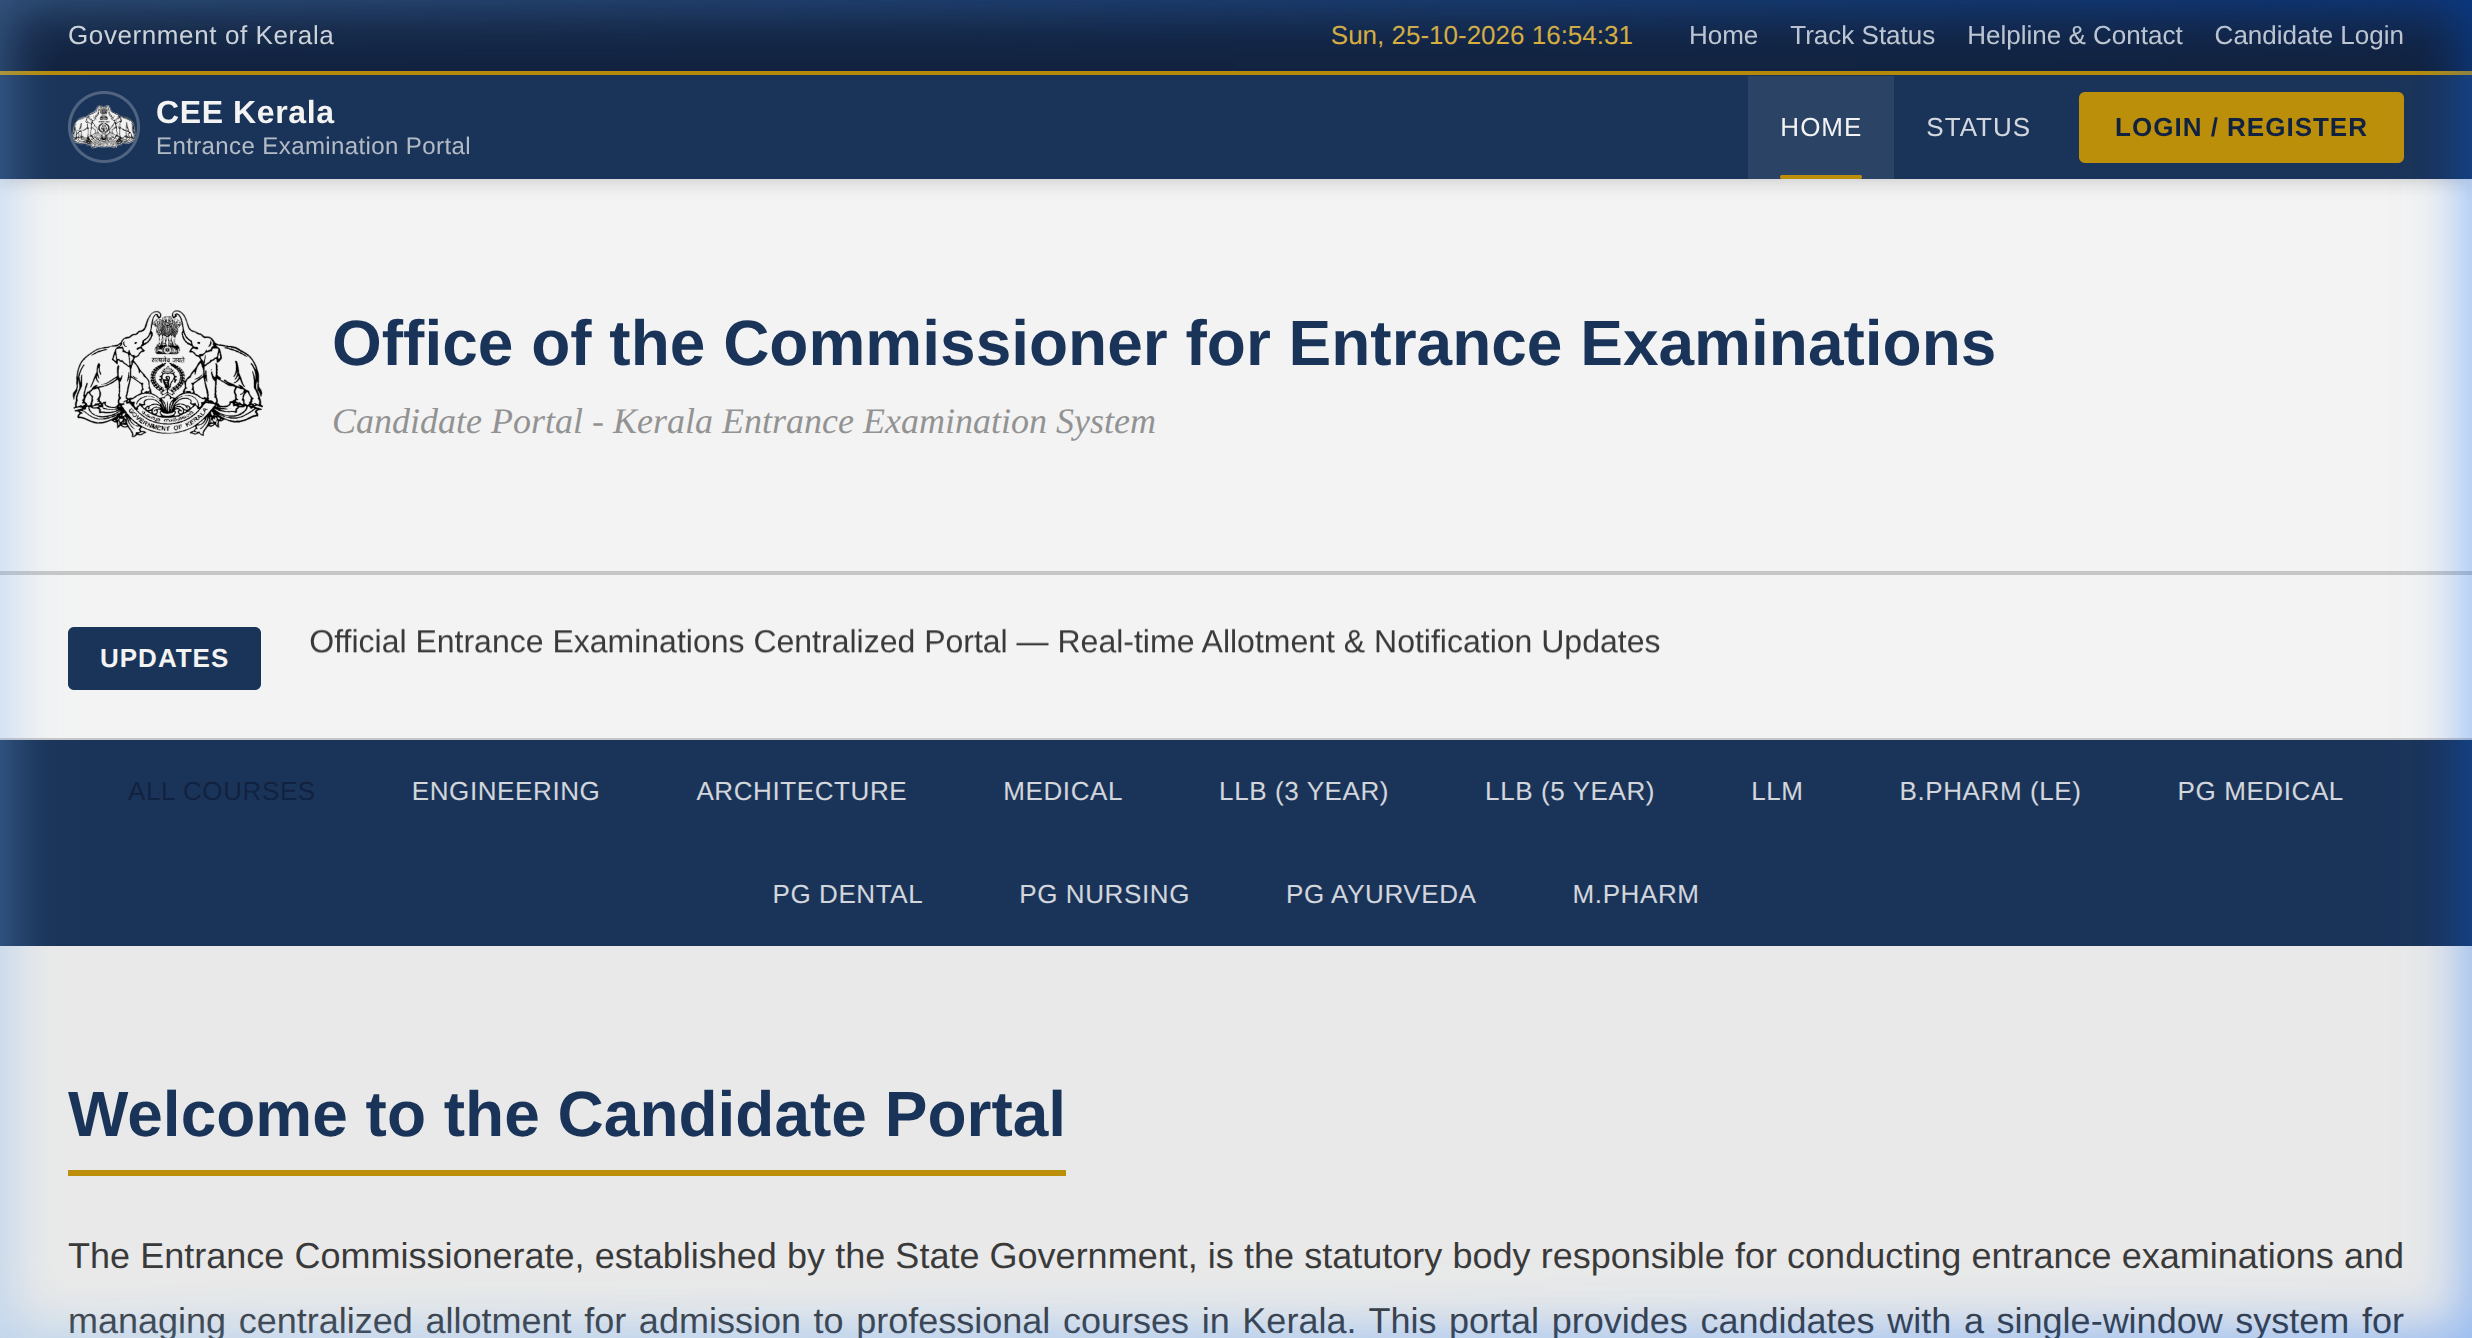
\includegraphics[width=0.88\textwidth,height=0.65\textheight,keepaspectratio]{images/landing_page.png}
\caption{KEAM Portal Landing Page with Government Band and Scrolling Ticker}
\label{fig:landing}
\end{figure}

Figure~\ref{fig:landing} displays the landing interface featuring the official government band, live digital clock, CEE emblem, navigation links, and dynamic scrolling announcement ticker.

\begin{figure}[!htbp]
\centering
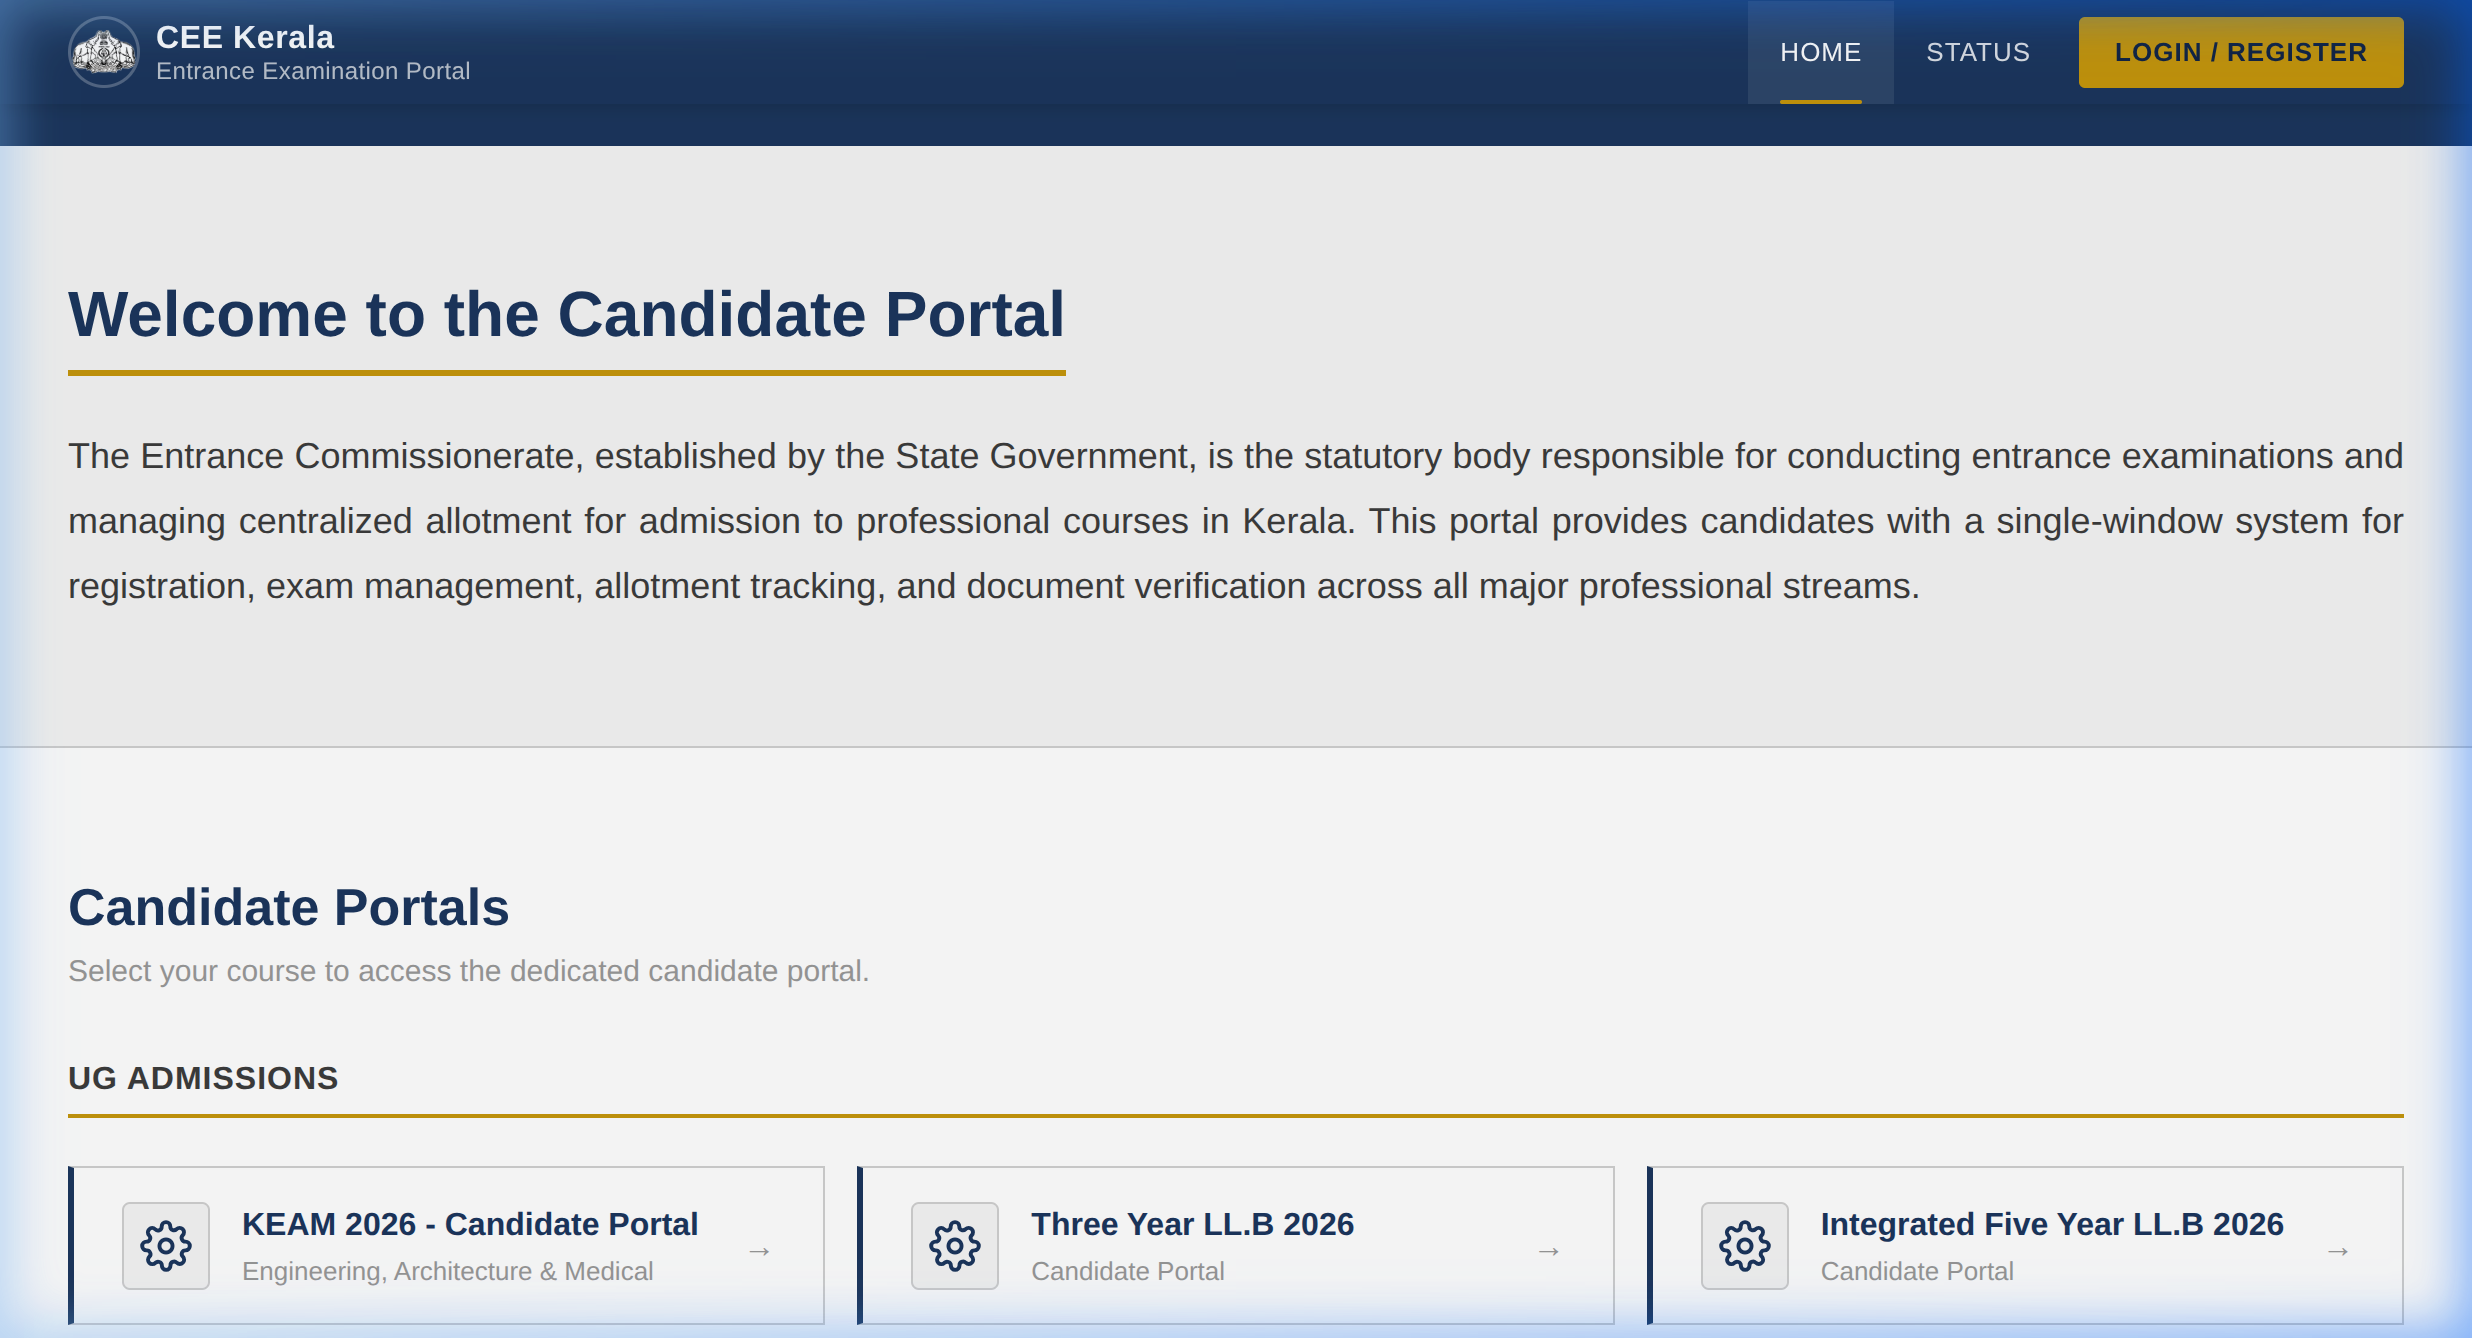
\includegraphics[width=0.88\textwidth,height=0.65\textheight,keepaspectratio]{images/landing_page_cards.png}
\caption{Portal Feature Cards and Examination Stream Tabs}
\label{fig:cards}
\end{figure}

Figure~\ref{fig:cards} illustrates the course-selection tabs and quick-access cards for registration, status tracking, and prospectus information.

\begin{figure}[!htbp]
\centering
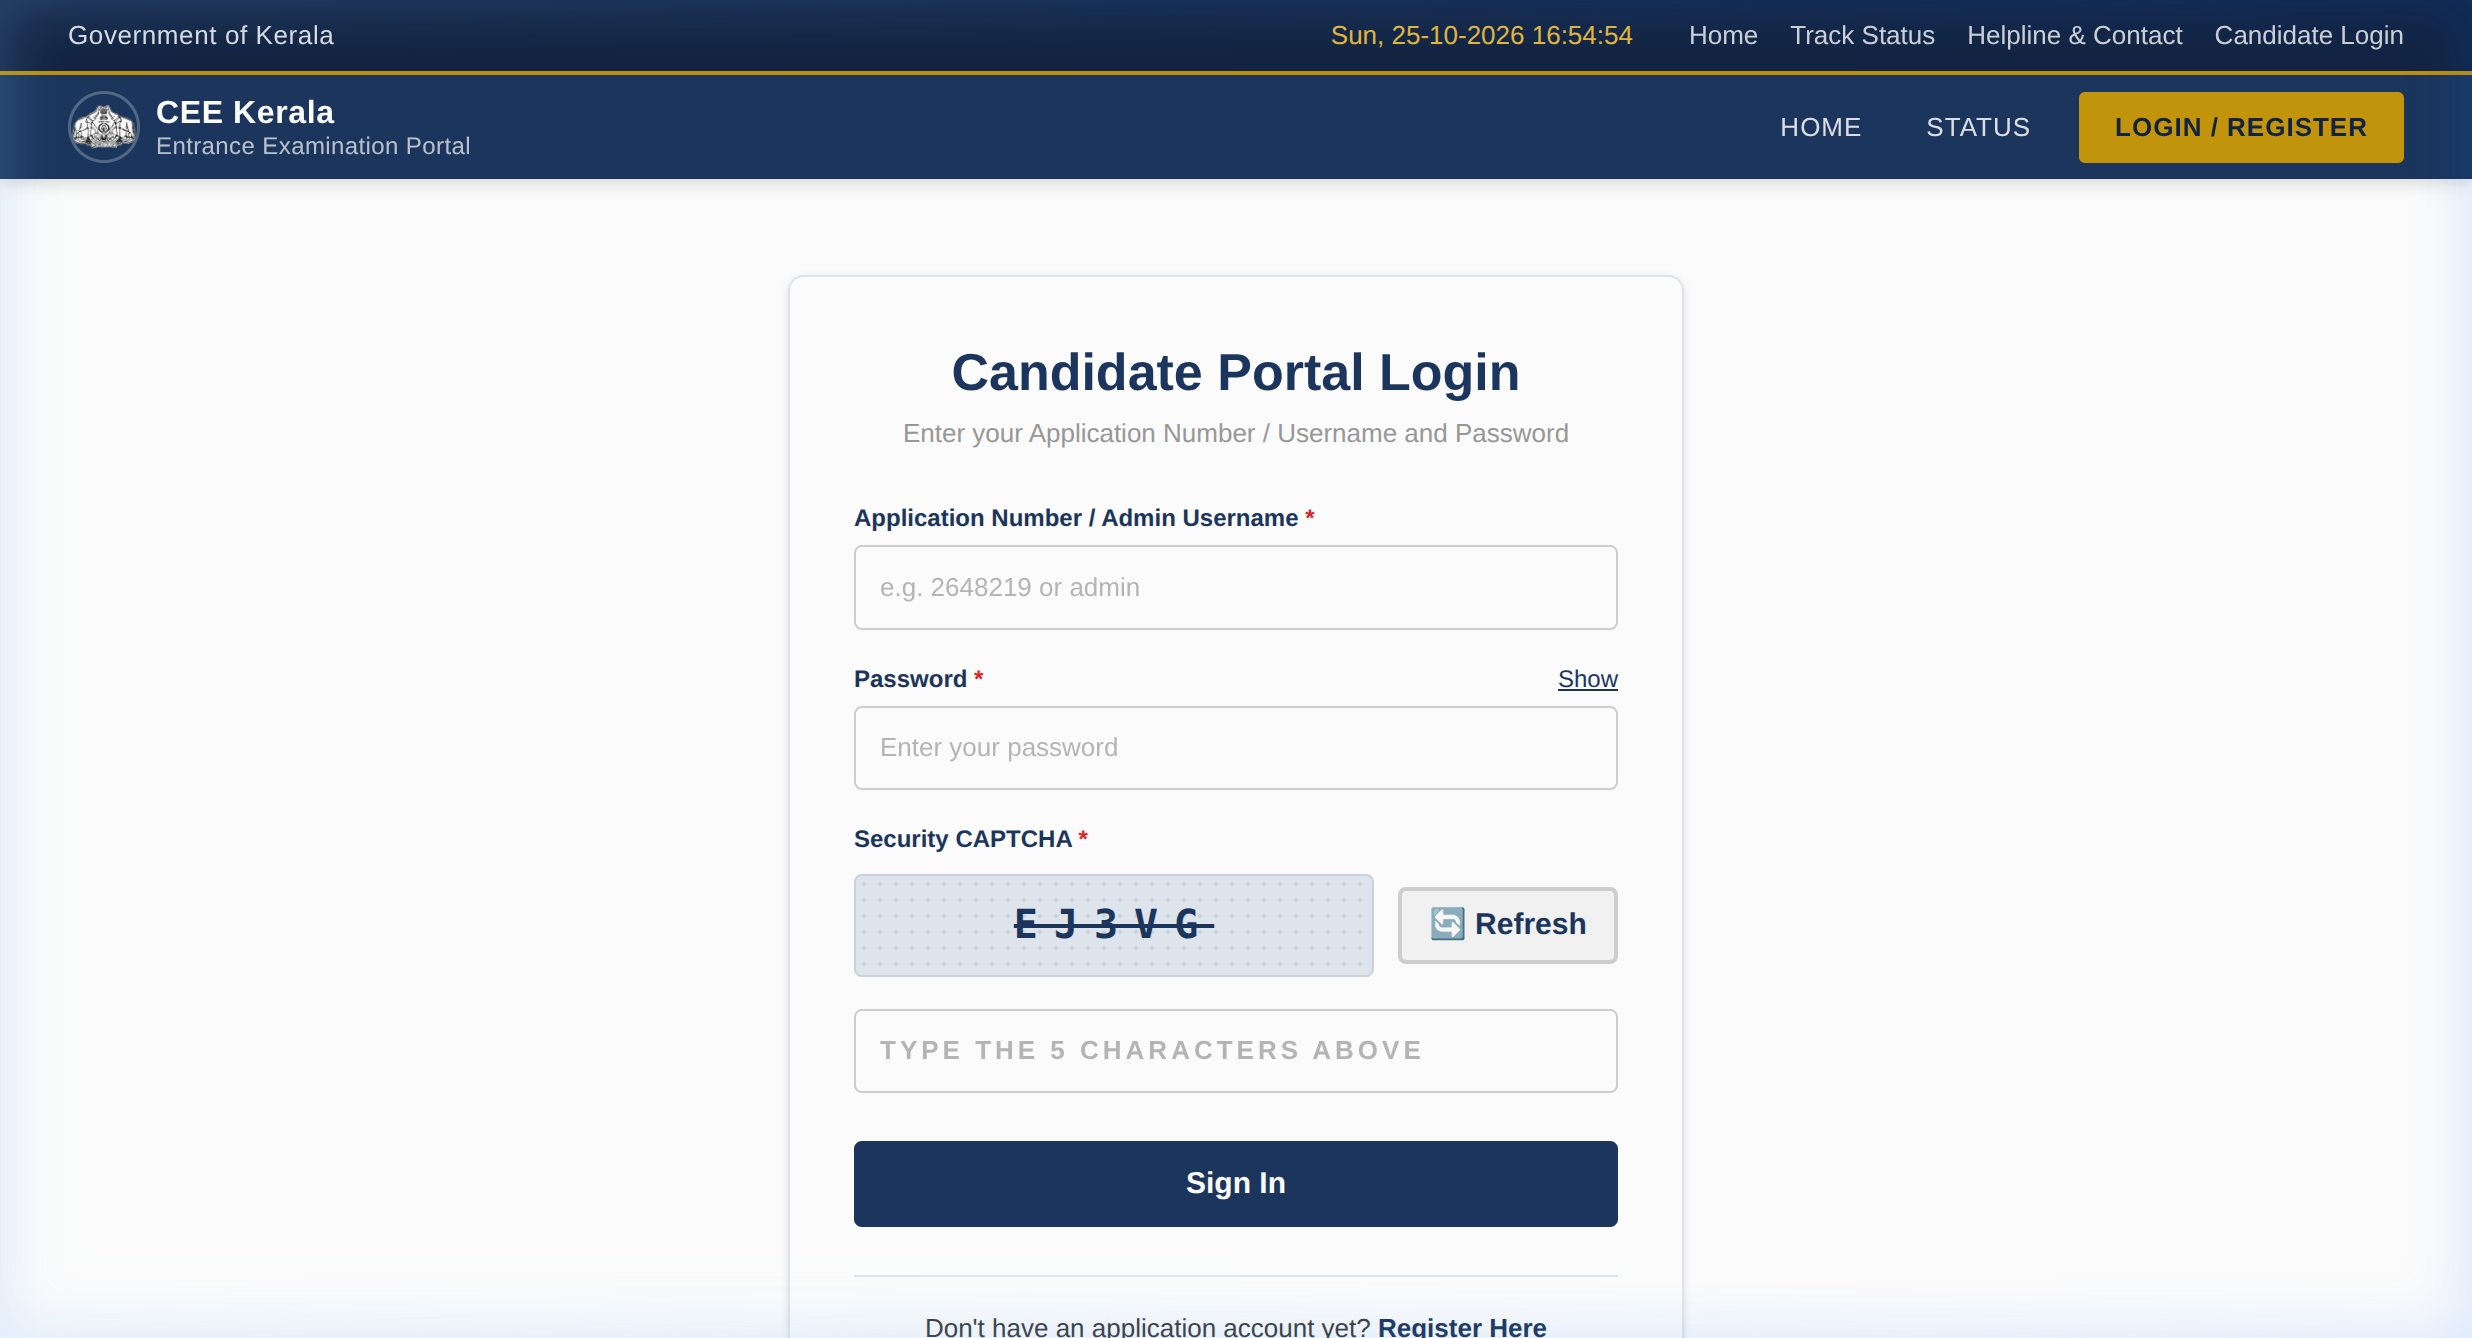
\includegraphics[width=0.65\textwidth,height=0.60\textheight,keepaspectratio]{images/login_page.png}
\caption{Candidate and Administrator Authentication Screen with CAPTCHA}
\label{fig:login}
\end{figure}

Figure~\ref{fig:login} shows the unified login interface for candidates and administrators, including CAPTCHA verification and password visibility controls.

\begin{figure}[!htbp]
\centering
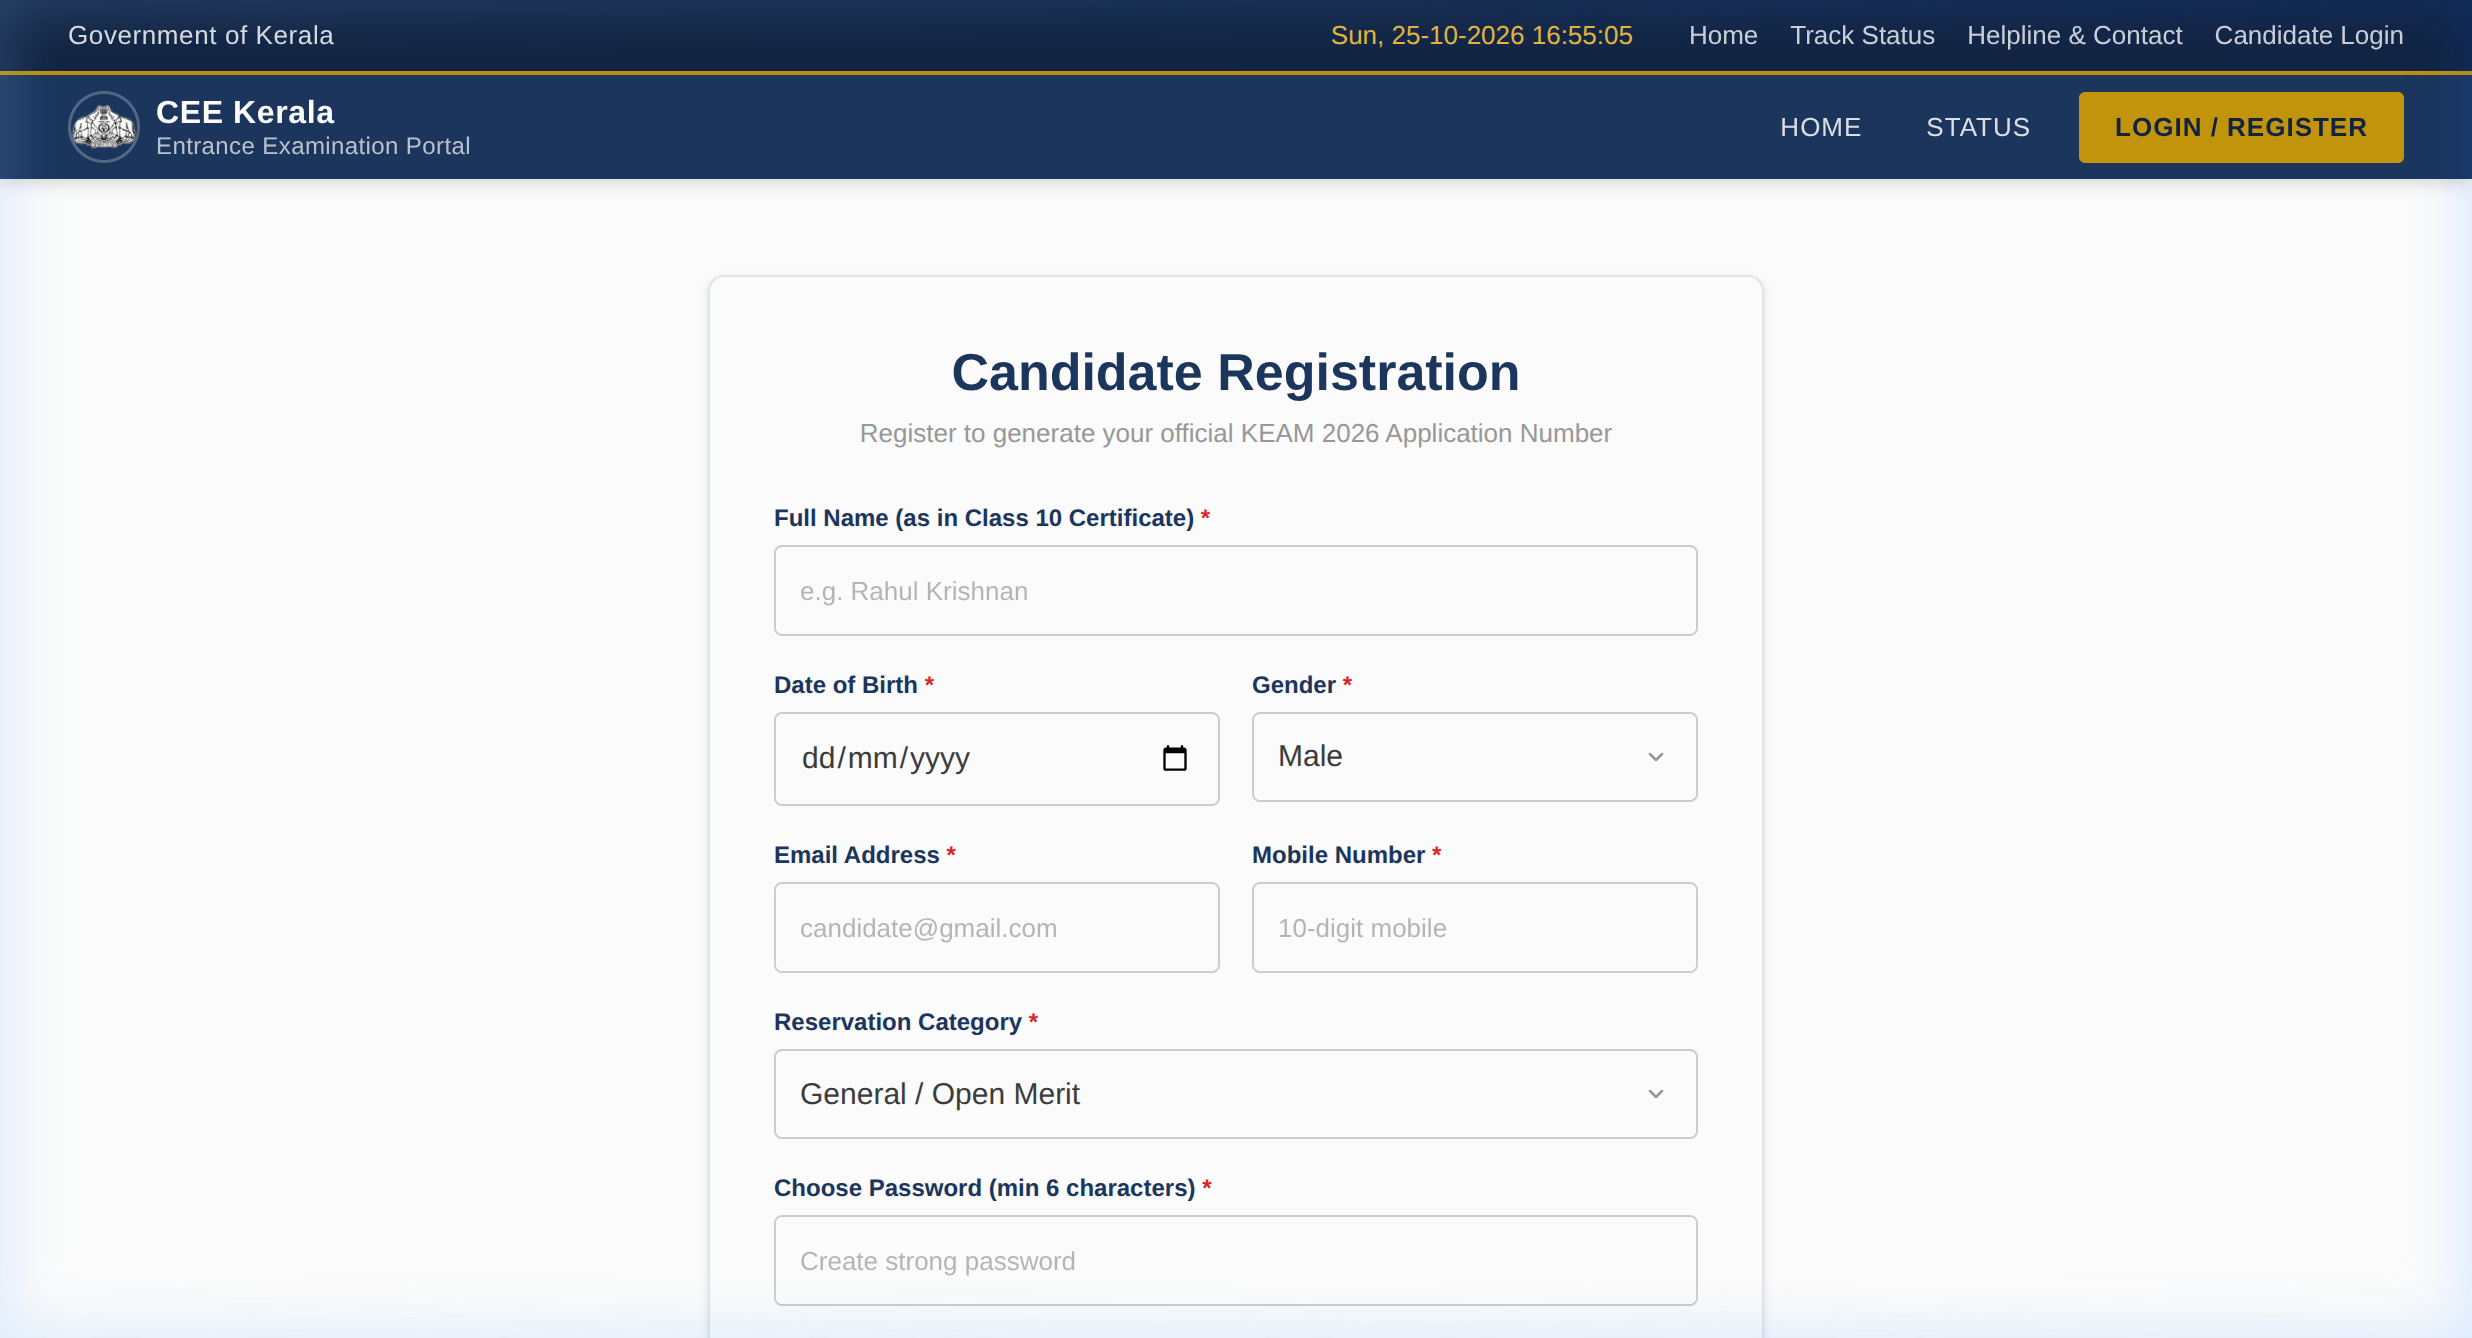
\includegraphics[width=0.72\textwidth,height=0.60\textheight,keepaspectratio]{images/register_page.png}
\caption{Candidate Registration Interface with Validation}
\label{fig:register}
\end{figure}

\begin{figure}[!htbp]
\centering
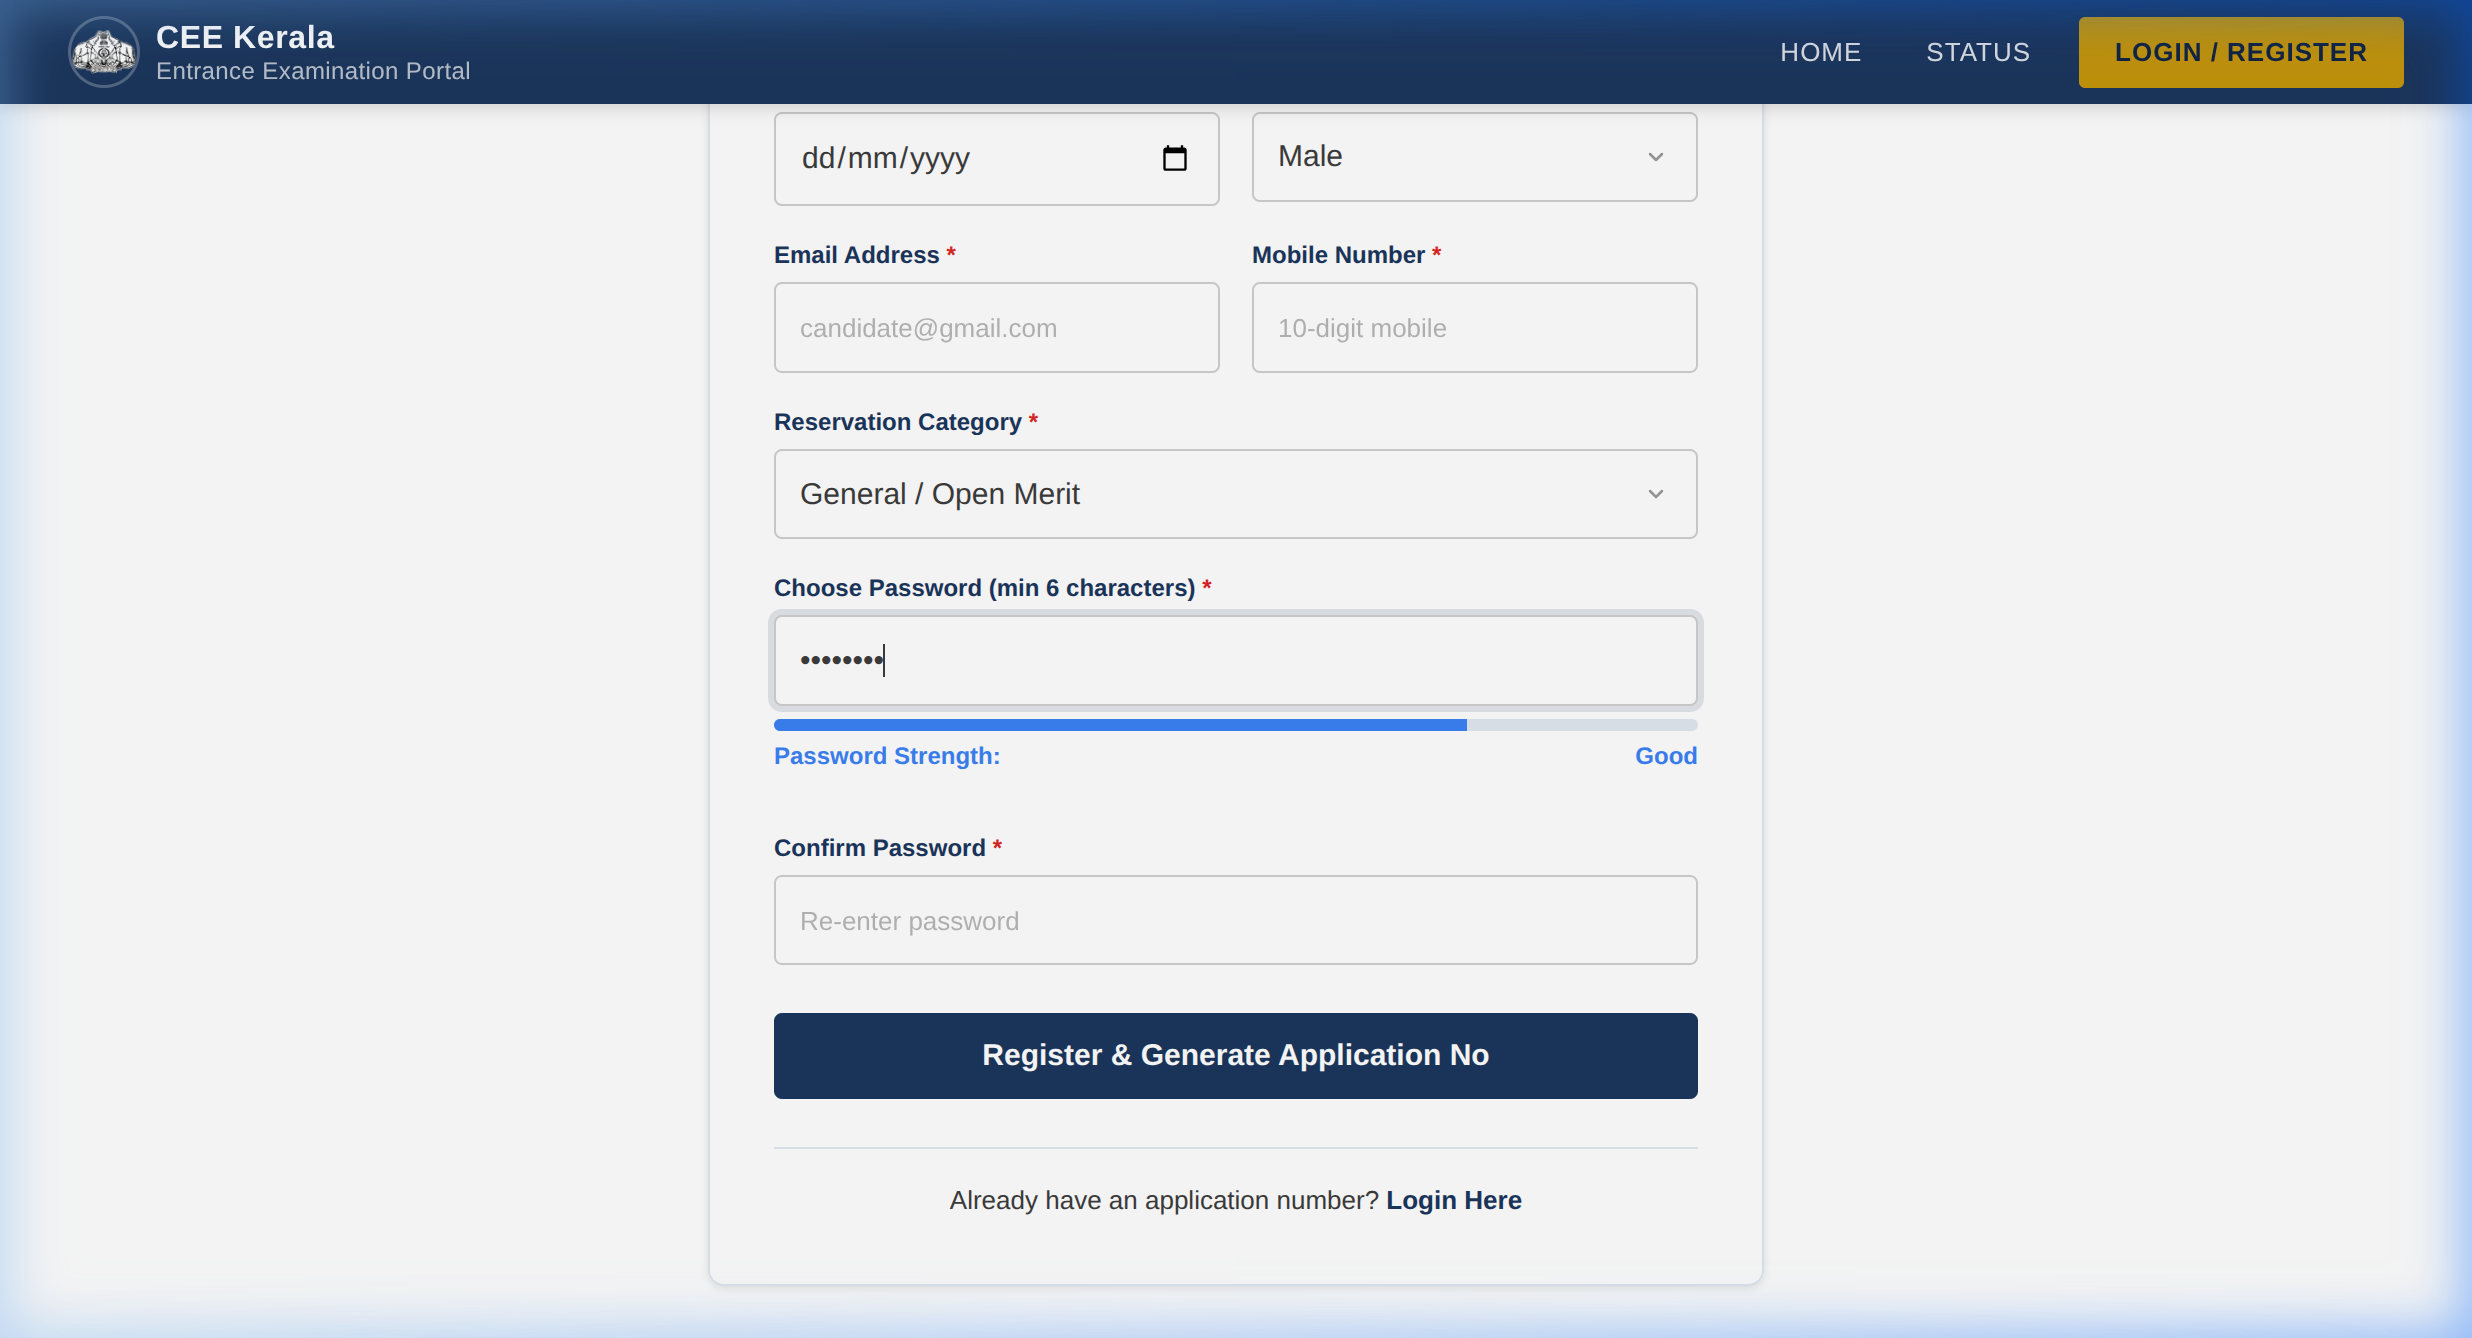
\includegraphics[width=0.68\textwidth,height=0.55\textheight,keepaspectratio]{images/password_meter.png}
\caption{Password Strength Visualizer}
\label{fig:pwdmeter}
\end{figure}

Figures~\ref{fig:register} and~\ref{fig:pwdmeter} demonstrate the candidate registration form with controlled inputs and the dynamic real-time password-strength meter.

\begin{figure}[!htbp]
\centering
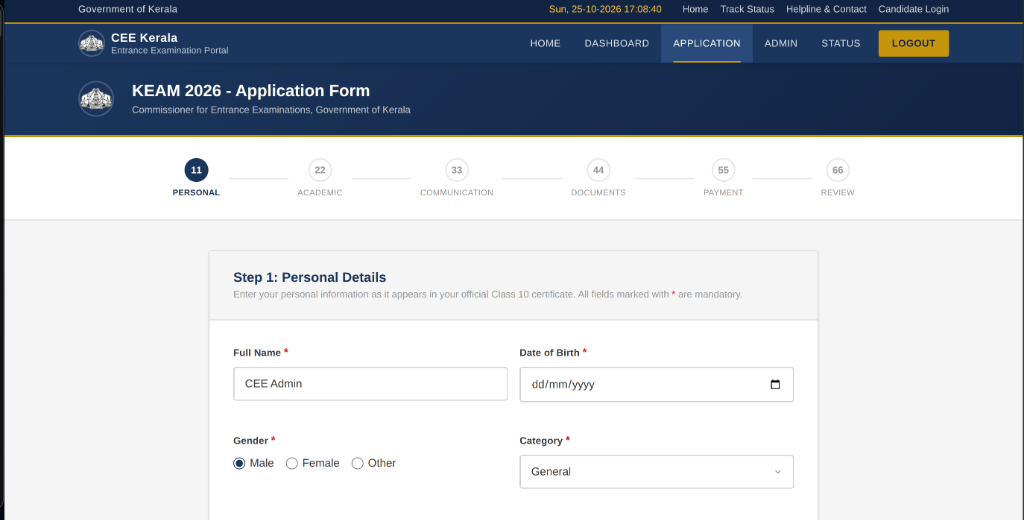
\includegraphics[width=0.85\textwidth,height=0.60\textheight,keepaspectratio]{images/application_form.png}
\caption{Six-Step Application Form Wizard}
\label{fig:wizard}
\end{figure}

Figure~\ref{fig:wizard} depicts the multi-step application wizard and its progress stepper. Form values are managed through hoisted parent state.

\begin{figure}[!htbp]
\centering
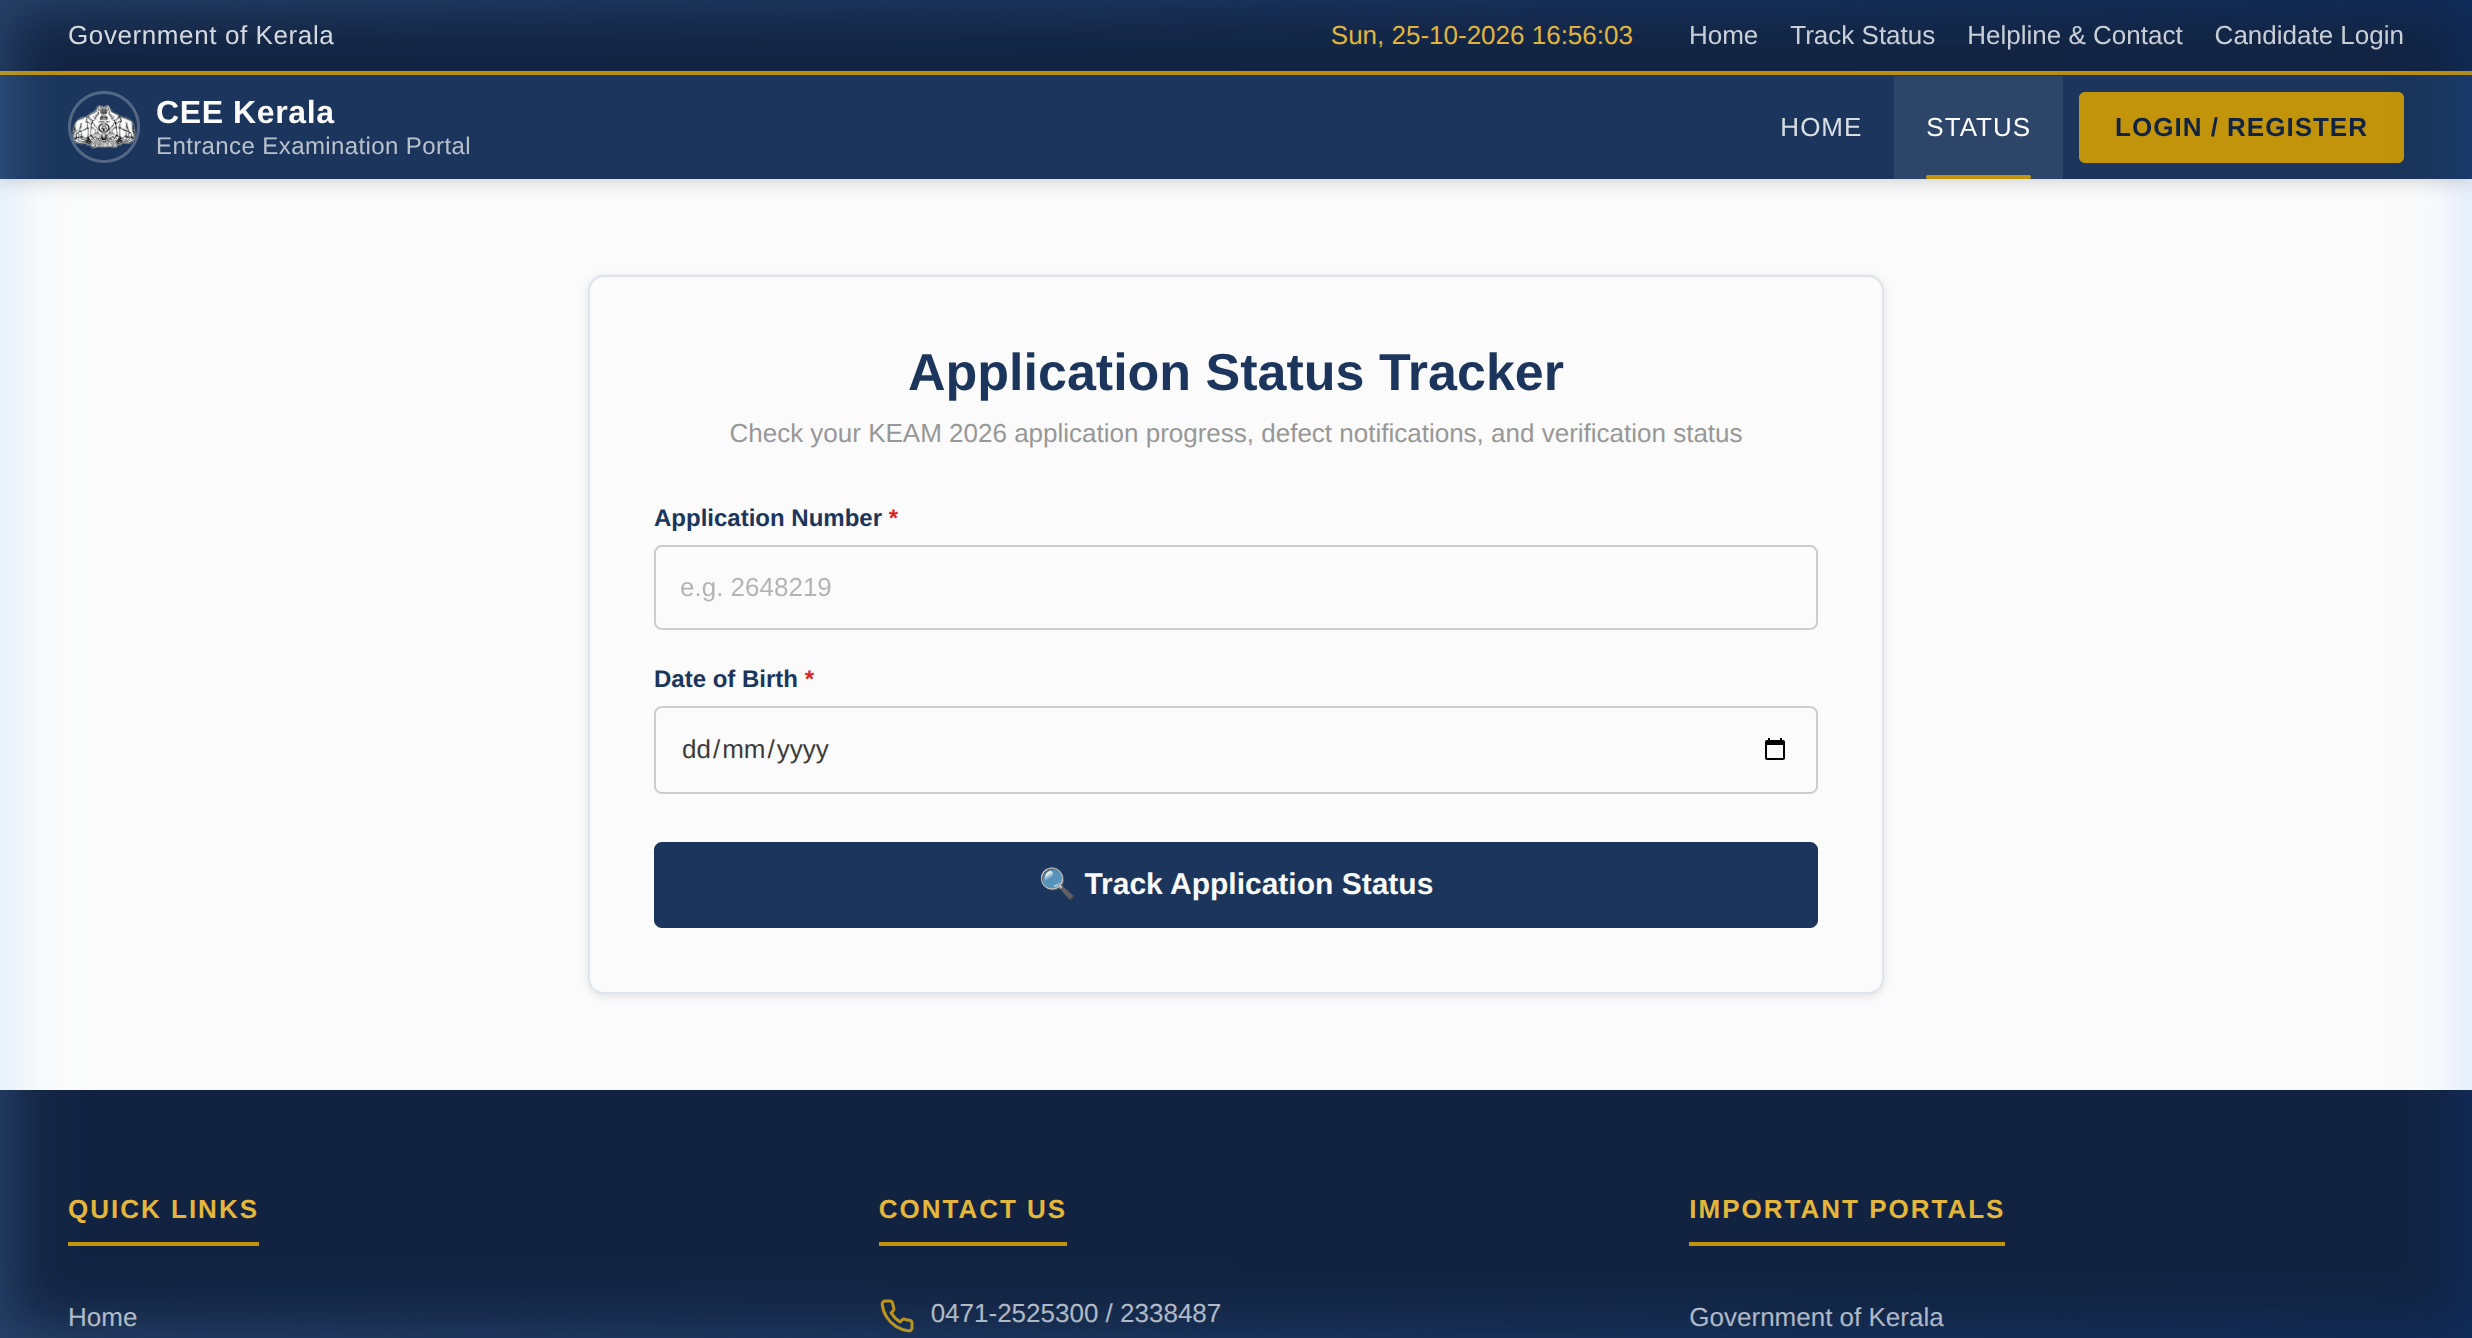
\includegraphics[width=0.75\textwidth,height=0.60\textheight,keepaspectratio]{images/status_page.png}
\caption{Public Application Milestone Status Tracker}
\label{fig:status}
\end{figure}

Figure~\ref{fig:status} shows the public status-tracking view where a candidate queries real-time verification decisions using application number and date of birth.

\begin{figure}[H]
\centering
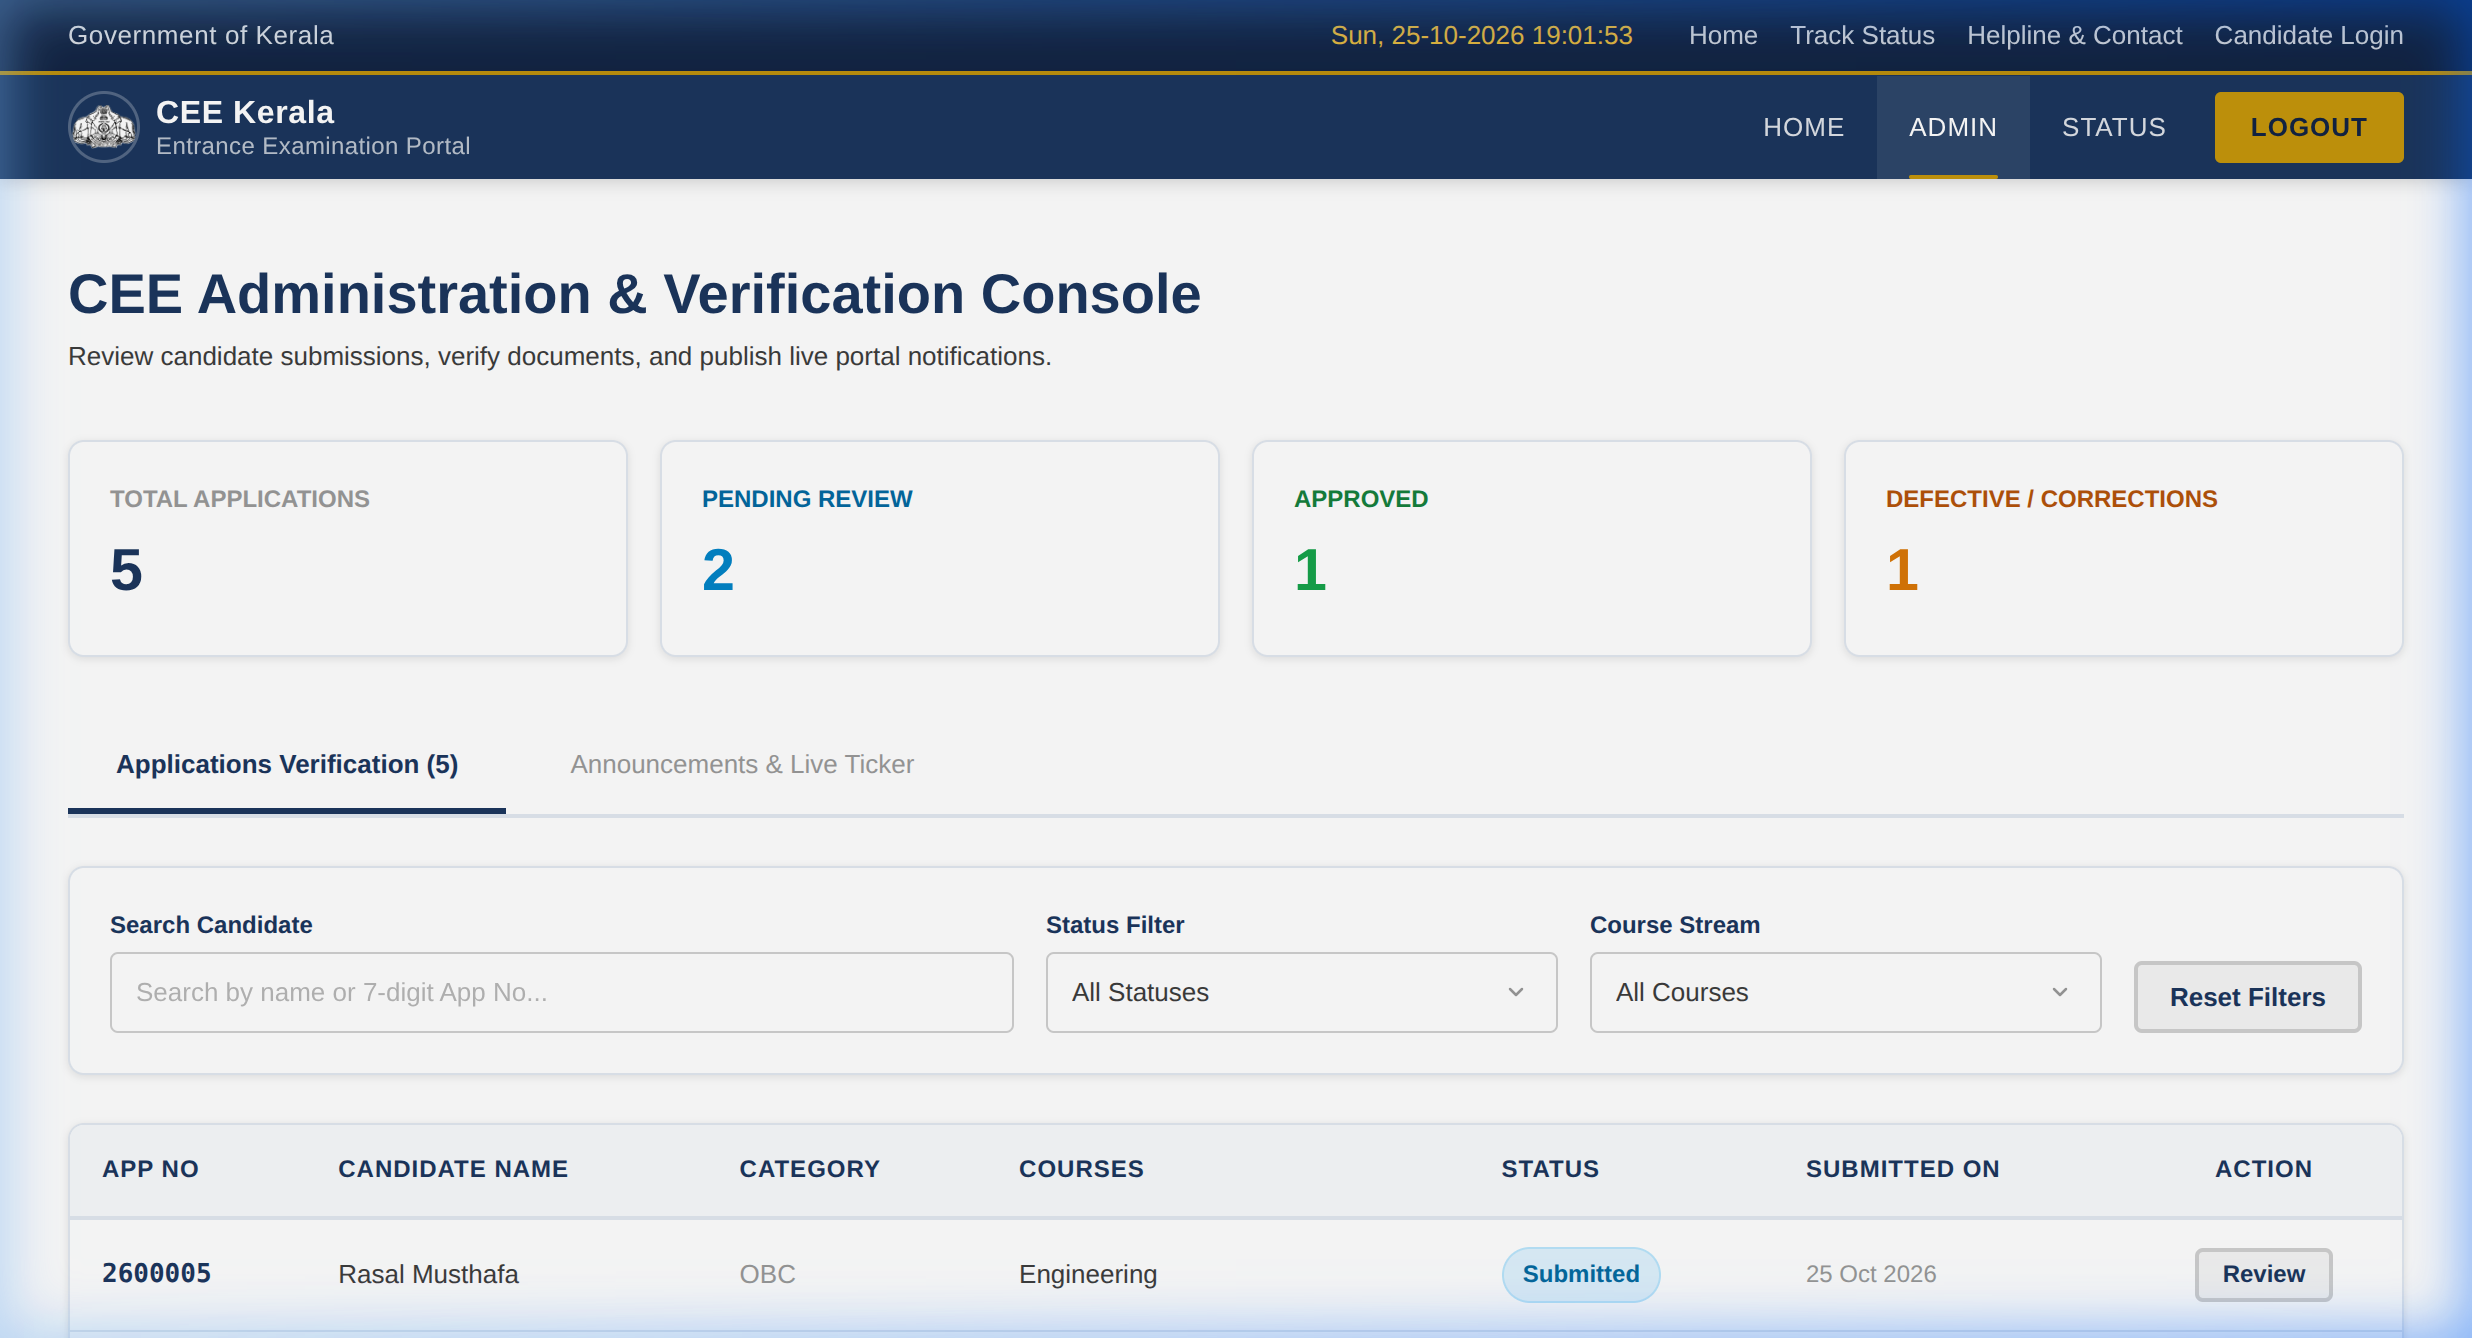
\includegraphics[width=0.92\textwidth,height=0.60\textheight,keepaspectratio]{images/admin_portal.png}
\caption{Administrator Application Scrutiny and Verification Console}
\label{fig:admin}
\end{figure}

Figure~\ref{fig:admin} displays the administrator dashboard with candidate application records, search and filter controls, status indicators, and review actions.

\begin{figure}[!htbp]
\centering
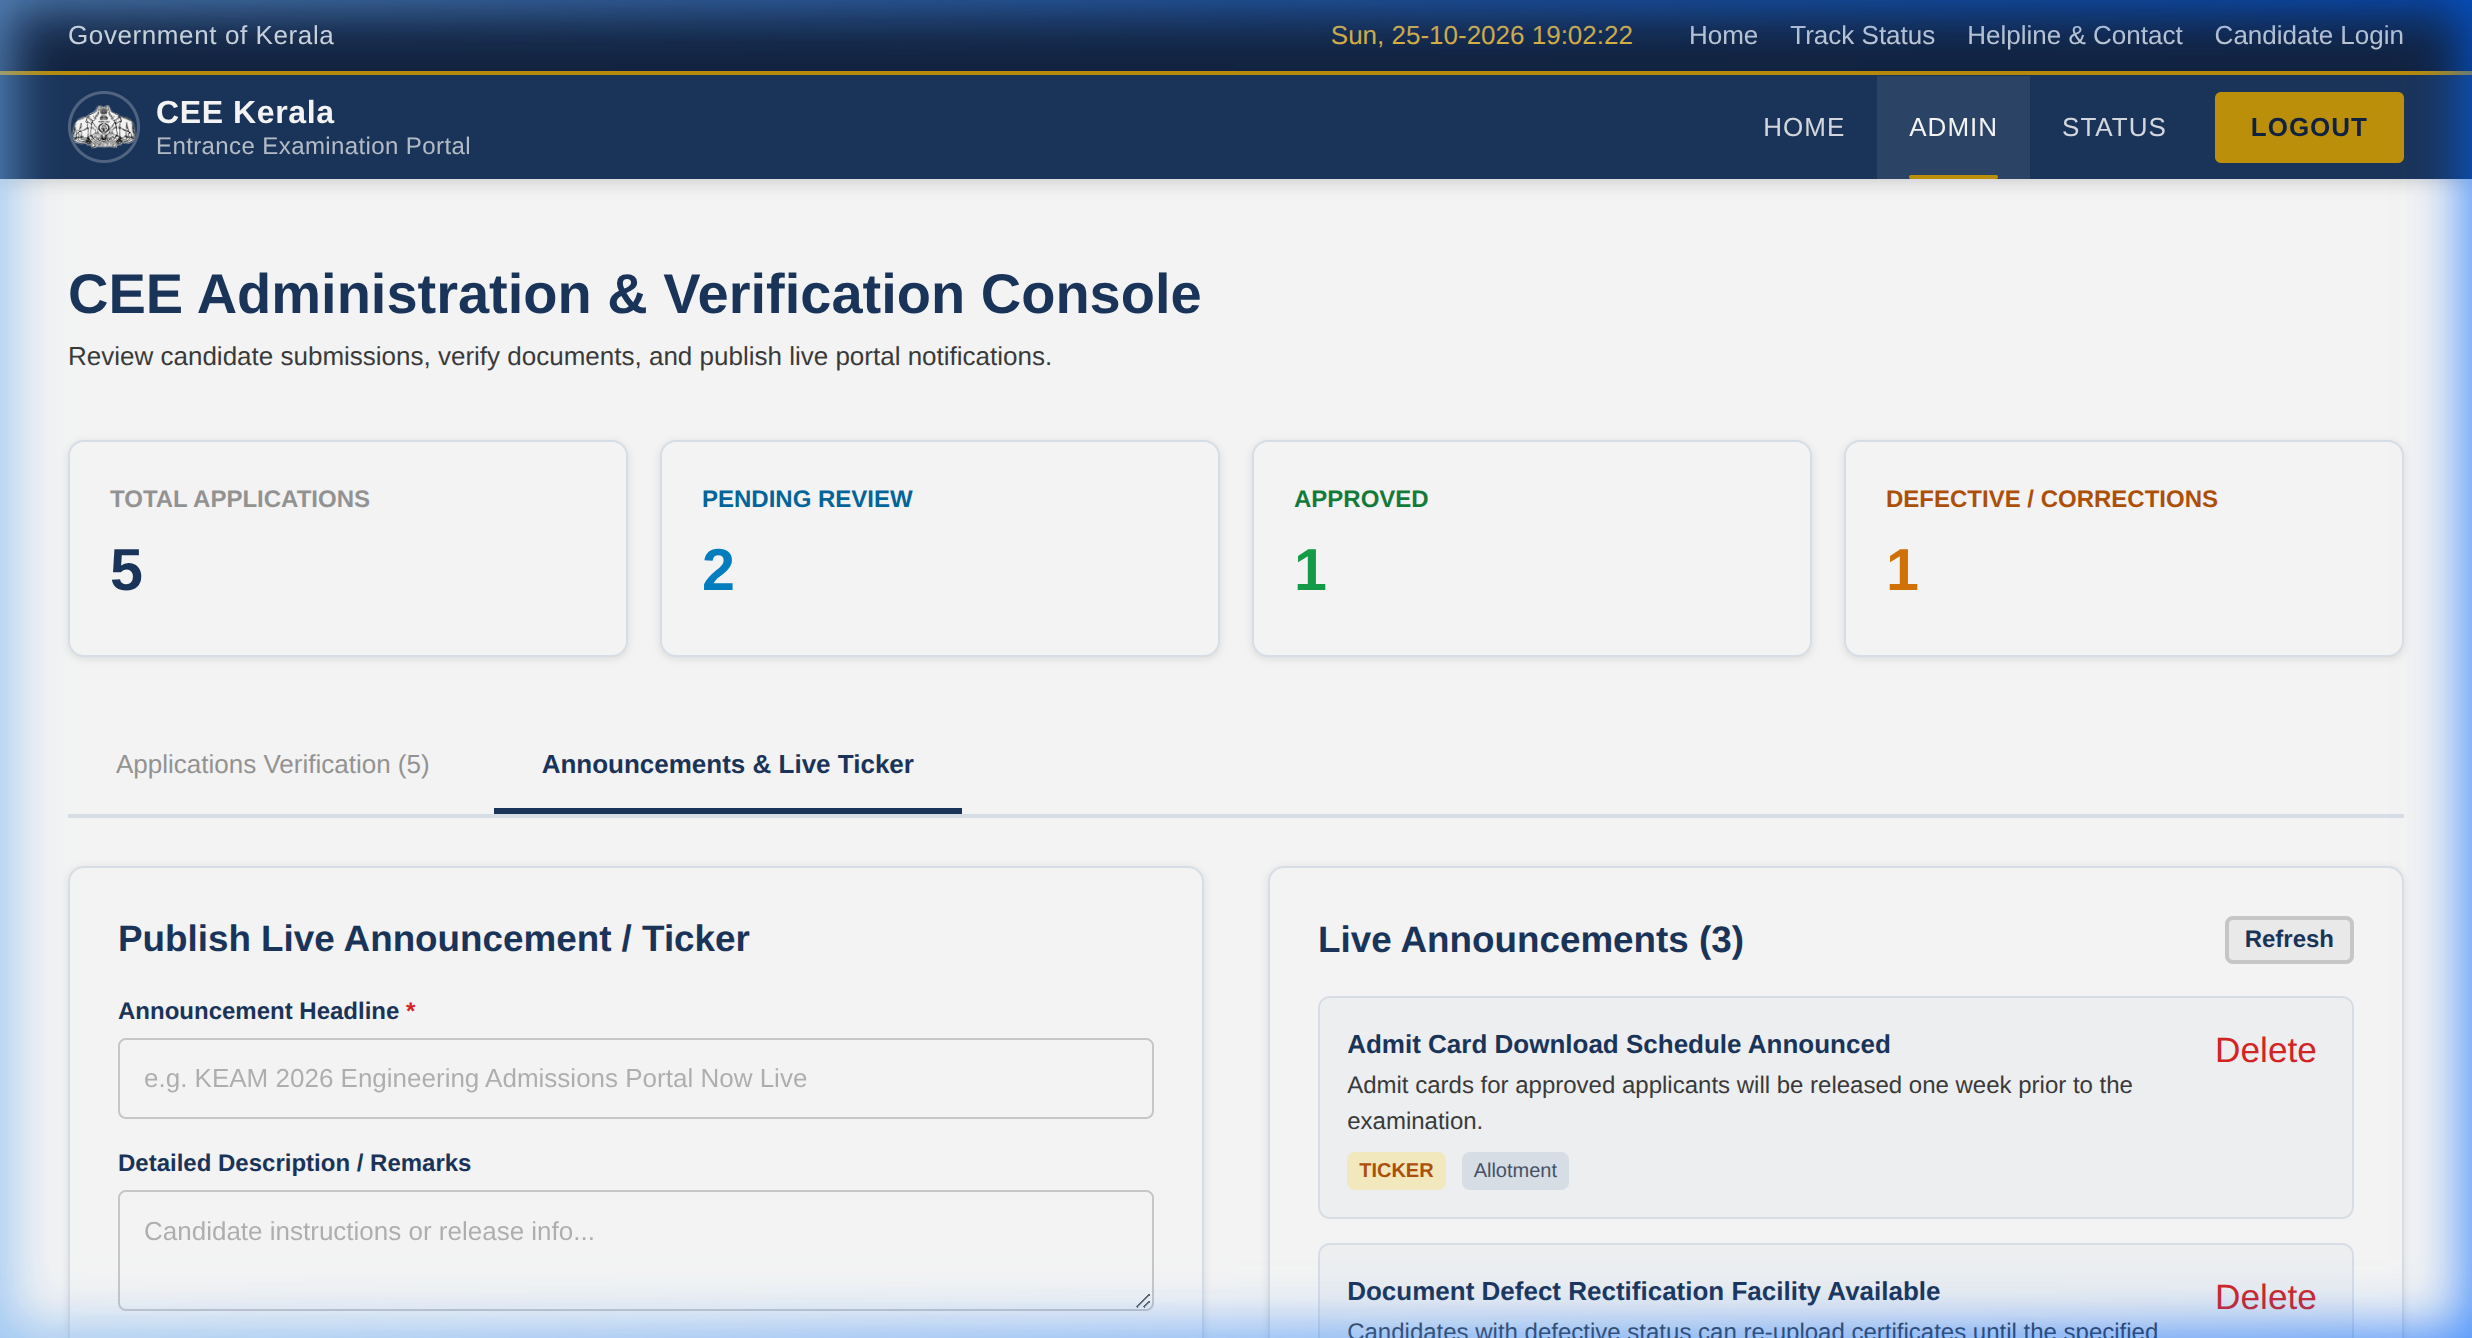
\includegraphics[width=0.92\textwidth,height=0.60\textheight,keepaspectratio]{images/admin_announcements.png}
\caption{Announcement and Scrolling Ticker Manager}
\label{fig:announcements}
\end{figure}

Figure~\ref{fig:announcements} shows the administrator interface for managing portal notices and scrolling announcements.

\section{Evaluation Rubric Compliance}
The project was evaluated against the standardized 20-mark React UI Project Evaluation Rubric across all five criteria. Table~\ref{tab:rubric} summarizes the technical mapping and evidence.

\begin{table}[!htbp]
\centering
\caption{React UI Project Evaluation Rubric Compliance Summary (20 Marks)}
\label{tab:rubric}
\small
\begin{tabularx}{\textwidth}{L{3.2cm} L{2.2cm} Y c}
\toprule
\textbf{Criterion} & \textbf{Target Level} & \textbf{Codebase Evidence and Implementation} & \textbf{Marks} \\
\midrule
1. Component Design \& Rendering & Excellent (4) & Pure functional components; reusable \texttt{InputField}, \texttt{SelectField}, and \texttt{Button}; conditional rendering in Navbar and step wizards. & 4 / 4 \\
2. UI Styling \& Responsiveness & Excellent (4) & Centralized design tokens in \texttt{index.css}; dynamic state styling in \texttt{PasswordStrength}; responsive media queries across viewports. & 4 / 4 \\
3. Hooks \& State Management & Excellent (4) & Correct usage of \texttt{useState}, \texttt{useEffect} with \texttt{clearInterval} cleanup in \texttt{DigitalClock}, Lifting State Up, and \texttt{AuthContext}. & 4 / 4 \\
4. Routing \& Forms & Excellent (4) & React Router v6 with \texttt{ProtectedRoute} guards; controlled inputs with live validation; async submission and error alert handling. & 4 / 4 \\
5. Individual Understanding & Excellent (4) & Clear modular architecture divided across five team members; independent problem solving and verifiable git contributions. & 4 / 4 \\
\midrule
\textbf{Total Score} & & & \textbf{20 / 20} \\
\bottomrule
\end{tabularx}
\end{table}

\section{Key Outcomes}
The implemented features demonstrate the following primary outcomes:
\begin{itemize}
    \item \textbf{Multi-step form persistence:} Hoisted React state retains form values while moving forward and backward across wizard steps.
    \item \textbf{Real-time search and filtering:} Instant client-side filtering supports rapid scrutiny of candidate records.
    \item \textbf{Role-based route guarding:} Unauthenticated visitors and non-admin users are automatically redirected from restricted candidate and administrator routes.
    \item \textbf{Scrutiny feedback loop:} Administrator remarks and defect flags are immediately reflected on the candidate-facing status tracker.
\end{itemize}

% =========================================================
% CHAPTER 7: CONCLUSION
% =========================================================
\chapter{Conclusion}

The \textbf{KEAM Portal Clone} project demonstrates the design and implementation of a full-stack web application inspired by an entrance examination and admission portal. Using MongoDB Atlas, Express.js, React.js, and Node.js, the project applies modern single-page application concepts to form handling, authentication, application review, and announcements.

The development process covered a responsive user interface, a RESTful backend, database schemas, bcrypt password hashing, JWT-based authorization, and a six-step application wizard. The administrator console provides application review and announcement management functions, while the candidate-facing interface presents application status information. The project demonstrates modern web-development practices, modular code organization, and collaborative engineering. It is an academic prototype and does not represent or replace the official KEAM portal.

% =========================================================
% CHAPTER 8: FUTURE SCOPE
% =========================================================
\chapter{Future Scope}

Potential future enhancements include:
\begin{enumerate}
    \item \textbf{Cloud deployment and containerization:} Package frontend and backend services in Docker containers and deploy them to a cloud platform with automated CI/CD pipelines.
    \item \textbf{Assisted document scrutiny:} Integrate OCR tools such as Tesseract or a cloud vision service to extract document text and flag possible quality issues for human review.
    \item \textbf{Multi-factor authentication:} Add email or SMS one-time passwords for account verification and password recovery.
    \item \textbf{Payment gateway integration:} Connect a live payment gateway and validate webhook signatures for fee reconciliation.
    \item \textbf{Rank list and allotment simulation:} Build a configurable demonstration of score normalization, reservation quota processing, and multi-round seat allotment.
    \item \textbf{Automated testing:} Implement end-to-end testing with Cypress or Playwright to automate regression testing across all application wizard steps.
\end{enumerate}

% =========================================================
% CHAPTER 9: MAPPING TO PROGRAM OUTCOMES AND SDGS
% =========================================================
\chapter{Mapping to Program Outcomes and SDGs}

\section{Mapping to Program Outcomes (POs)}
\begin{itemize}
    \item \textbf{PO1 - Engineering Knowledge:} Applied computing, client-server networking, REST architecture, and database concepts.
    \item \textbf{PO2 - Problem Analysis:} Identified admission workflow challenges and translated them into functional software specifications.
    \item \textbf{PO3 - Design/Development of Solutions:} Designed a multi-step form wizard, role-based route guards, and scrutiny review modules.
    \item \textbf{PO5 - Modern Tool Usage:} Used React.js 18, Vite 5, Node.js v24, Express.js, MongoDB Atlas, Git, GitHub, VS Code, and Postman.
    \item \textbf{PO8 - Individual and Team Work:} Distributed work systematically across a five-member team covering frontend, backend, authentication, and administration.
    \item \textbf{PO9 - Communication:} Prepared technical documentation and a formal project report.
    \item \textbf{PO10 - Project Management:} Coordinated development tasks and milestones across three distinct project phases.
    \item \textbf{PO12 - Life-Long Learning:} Developed proficiency with modern web frameworks and development workflows through self-directed investigation.
\end{itemize}

\section{Mapping to Sustainable Development Goals (SDGs)}
\begin{itemize}
    \item \textbf{SDG 4 - Quality Education:} Demonstrates a digital workflow intended to make admission information and application status transparent and accessible.
    \item \textbf{SDG 9 - Industry, Innovation, and Infrastructure:} Applies modern web technologies to build resilient digital public-service infrastructure.
    \item \textbf{SDG 11 - Sustainable Cities and Communities:} Demonstrates online workflows that eliminate unnecessary physical visits to administrative offices.
    \item \textbf{SDG 12 - Responsible Consumption and Production:} Promotes paperless processing for application forms, uploads, and notices.
\end{itemize}

% =========================================================
% CHAPTER 10: REFERENCES
% =========================================================
\chapter{References}
\begin{enumerate}
    \item React Documentation. \textit{React: The Library for Web and Native User Interfaces}. Available: \url{https://react.dev}
    \item Node.js. \textit{Node.js Documentation}. Available: \url{https://nodejs.org/docs}
    \item Express.js. \textit{Express Web Framework Documentation}. Available: \url{https://expressjs.com}
    \item MongoDB, Inc. \textit{MongoDB Documentation}. Available: \url{https://www.mongodb.com/docs}
    \item Vite. \textit{Vite Documentation}. Available: \url{https://vite.dev}
    \item Commissioner for Entrance Examinations, Kerala. \textit{Official CEE Kerala Website}. Available: \url{https://cee.kerala.gov.in}
    \item United Nations. \textit{The 17 Sustainable Development Goals}. Available: \url{https://sdgs.un.org/goals}
    \item Internet Engineering Task Force. (2015). \textit{RFC 7519: JSON Web Token (JWT)}. Available: \url{https://datatracker.ietf.org/doc/html/rfc7519}
    \item Provos, N., and Mazieres, D. (1999). \textit{A Future-Adaptable Password Scheme (Bcrypt)}. USENIX Annual Technical Conference, FREENIX Track.
    \item MDN Web Docs. \textit{Web Documentation}. Available: \url{https://developer.mozilla.org}
    \item GitHub. \textit{GitHub Documentation}. Available: \url{https://docs.github.com}
\end{enumerate}

\end{document}
